%!TEX program = xelatex
\documentclass[12pt]{report}
\usepackage{amsmath, amssymb, amsthm, mathtools}
% \usepackage{tocbibind}
\usepackage[left=1.5in,right=1.5in,top=1.25in,bottom=1.25in]{geometry}
\usepackage{bm}
\usepackage{bbm}
\usepackage{fancyhdr}
\usepackage[nohyperlinks]{acronym}
\usepackage{algorithm}
\usepackage{algpseudocode}
\usepackage{datetime}
\usepackage{natbib}
\usepackage{enumitem}
\usepackage{float}
\usepackage{multirow}
% \usepackage{subfig}
\usepackage{subcaption}
\usepackage[normalem]{ulem}
%\usepackage[affil-it]{authblk}
%\usepackage[percent]{overpic}
%\usepackage{rotating}
\usepackage{tikz}
\usetikzlibrary{shapes,positioning,arrows,chains}

\definecolor{grey1}{HTML}{333333}
\definecolor{grey2}{HTML}{666666}
\definecolor{grey3}{HTML}{999999}
\definecolor{grey4}{HTML}{DDDDDD}
\definecolor{white}{HTML}{FFFFFF}
\definecolor{yellowLight}{HTML}{CCCC33}
\definecolor{yellowDark}{HTML}{808001}
\definecolor{magenta}{HTML}{A4296F}

\newcommand{\Z}[0]{\mathbb{Z}}
\newcommand{\R}[0]{\mathbb{R}}
\newcommand{\C}[0]{\mathbb{C}}
\newcommand{\B}[1]{\mathbf{#1}}
\newcommand{\m}[1]{\texttt{#1}}
\newcommand{\N}[0]{\mathbb{N}}
\newcommand{\F}[0]{\mathcal{F}}
\newcommand{\M}[2]{M_{#1 \times #2}}
\newcommand{\p}[0]{\prime}
\newcommand{\RV}[0]{\text{\textnormal{RV}}}
\newcommand{\st}[0]{\;\colon\;}
\newcommand{\tr}[0]{\text{\textnormal{tr}}}
\newcommand{\err}[0]{\text{\textnormal{err}}}
\newcommand{\poly}[0]{\text{\textnormal{poly}}}
\newcommand{\vcdim}[0]{\text{\textnormal{VCdim}}}
\newcommand{\E}[0]{\text{\textnormal{E}}}
\newcommand{\supp}[0]{\text{\textnormal{supp}}}
\newcommand{\suc}[0]{\text{\texttt{succ}}}
\newcommand{\1}[0]{\mathbbm{1}}

\newcommand{\Beta}[0]{\textnormal{Beta}}
\newcommand{\Unif}[0]{\textnormal{Unif}}
\newcommand{\Cat}[0]{\textnormal{Cat}}
\newcommand{\Dir}[0]{\textnormal{Dir}}
\newcommand{\Bern}[0]{\textnormal{Bern}}
\newcommand{\Norm}[0]{\textnormal{Norm}}
\newcommand{\SomeDist}[0]{\textnormal{D}}
\newcommand{\GEM}[0]{\textnormal{GEM}}
\newcommand{\HMM}[0]{\textnormal{HMM}}
\newcommand{\Geom}[0]{\textnormal{Geom}}

\newcommand{\Bf}[0]{\text{\textbf{B}}}
\newcommand{\seq}[3]{\ensuremath{#1_{{#2}:{#3}}}}

% \newcommand{\seq}[3]{\ensuremath{#1_{#2}(#3)}}
% \newcommand{\seq}[3]{\ensuremath{\{#1\}_{#2}^{#3}}}


\newcommand{\msout}[1]{\text{\sout{\ensuremath{#1}}}}

\renewcommand*{\Pr}{\text{\textnormal{P}}}
\renewcommand{\qedsymbol}{$\blacksquare$}
\DeclarePairedDelimiter\abs{\lvert}{\rvert}%
\DeclarePairedDelimiter\norm{\lVert}{\rVert}%
\DeclarePairedDelimiter{\ceil}{\lceil}{\rceil}
\DeclarePairedDelimiter{\floor}{\lfloor}{\rfloor}
\renewcommand{\dateseparator}{.}

\tikzset{randvar/.style={circle,draw,minimum size=30pt,inner sep=0pt,line width=1pt}}
\tikzset{gate/.style={circle,fill=black,draw,minimum size=10pt,inner sep=0pt,line width=1pt}}

\tikzset{textbox/.style={draw=none,color=black,font=\tiny}}
\tikzset{cover/.style={rectangle,draw,color=grey2,fill=grey2}}

\tikzset{input/.style={rectangle,color=white,draw,minimum height=60pt,minimum width=5pt,line width=1pt,font=\tiny,text width=2pt}}
\tikzset{output/.style={circle,color=white,draw,minimum size=20pt,inner sep=0cm,line width=1pt,font=\tiny}}

\tikzset{hinput/.style={rectangle,color=yellowLight,draw,minimum height=60pt,minimum width=5pt,line width=1pt,font=\tiny,text width=2pt}}
\tikzset{houtput/.style={circle,color=yellowLight,draw,minimum size=20pt,inner sep=0cm,line width=1pt,font=\tiny}}
\tikzset{htextbox/.style={draw=none,color=yellowLight,font=\tiny}}

\newcommand*\Let[2]{\State #1 $\gets$ #2}
\algrenewcommand\algorithmicrequire{\textbf{Input:}}
\algrenewcommand\algorithmicensure{\textbf{Output:}}

\setlength\parindent{0pt}

\author{Thomas L. Lake\\\normalsize{\emph{Western Michigan University}}\\\&\\\normalsize{\emph{Atlas Wearables}}}
\title{ANALYZING REPETITIVE SEQUENCES WITH STRUCTURED DYNAMIC BAYESIAN NETWORKS}
\date{\yyyymmdddate\today}

\begin{document}
\thispagestyle{empty}
\newgeometry{top=1.75in}
\begin{center}
    ANALYZING REPETITIVE SEQUENCES WITH STRUCTURED DYNAMIC BAYESIAN NETWORKS

    \vspace{3\baselineskip}
    Thomas L. Lake, M.S.

    \vspace{\baselineskip}
    Western Michigan University, 2015
\end{center}
\vspace{3\baselineskip}
\hspace*{0.5in}
Time series often feature structure that is known a priori and easily described using
natural language terms such as repetitive, symmetric, seasonal, and self-similar.
However, the typical conjugate priors used in Bayesian analysis do not capture such
complex phenomena well.
As a result of this mismatch, known structure is modeled poorly or completely ignored.
Focusing on time series with repetitive structure, this thesis proposes to overcome this
problem by reducing rather than increasing the capacity of a well know time series model,
the Hidden Markov Model.
Through a careful choice in the way model capacity is reduced the model is forced to use
its latent variables in an interpretable way which accurately reflects known structure.
In addition to increased modeling performance, the lower capacity model admits reduced
complexity inference and parameter estimation procedures.
Experimental results are presented demonstrating the effectiveness of this approach
in both supervised and unsupervised learning contexts.
\newpage
\restoregeometry

\pagenumbering{roman}
\thispagestyle{empty}
\newgeometry{top=1.75in}
\begin{center}
    \vspace{1.75in}
    ANALYZING REPETITIVE SEQUENCES WITH STRUCTURED DYNAMIC BAYESIAN NETWORKS

    \vspace{6\baselineskip}
    by

    \vspace{\baselineskip}
    Thomas L. Lake

    \vfill

    A dissertation submitted to the Graduate College\\
    in partial fulfillment of the requirements\\
    for the degree of Master of Science\\
    in Computer Science\\
    Western Michigan University\\
    December 2015
\end{center}
\vspace{10\baselineskip}
Thesis Committee:
\\\\
\hspace*{0.5in} Elise de Doncker, Ph.D., Chair\\
\hspace*{0.5in} Robert Trenary, Ph.D.\\
\hspace*{0.5in} John Kapenga, Ph.D.
\newpage
\restoregeometry


% \chapter*{Disclaimer}
% This document describes privately funded research intended
% for commercial use. Any redistribution of this document or the material
% contained within without express written consent of the author, Thom L. Lake,
% is in direct violation of terms agreed upon before receiving this document.
%
% \chapter*{Abstract}
% Time series often feature structure that is known a priori and easily described using
% natural language terms such as repetitive, symmetric, seasonal, and self-similar.
% However, the typical priors used in Bayesian analysis, normally due to the
% convenience of conjugacy, do not capture such complex phenomena well.
% As a result of this mismatch, known structure is modeled poorly or completely ignored.
% Focusing on time series with repetitive structure, this thesis proposes to overcome this
% problem by reducing, rather than increasing, the capacity of a well know time series model,
% the Hidden Markov Model.
% Through a careful choice in the way model capacity is reduced, the model is forced to use
% its latent variables in an interpretable way which accurately reflects known structure.
% In addition to increased modeling performance, the lower capacity model also admits more
% efficient inference and parameter estimation procedures.
% Experimental results are presented demonstrating the effectiveness of this approach both
% in a supervised and unsupervised learning context.

% \chapter*{Dedication}
% To my wife Brooke Lake.
%
% \chapter*{Declaration}
% I declare that this has taken too long
%
\chapter*{Acknowledgments}
I want to thank my advisor Elise deDoncker and Robert Trenary for all their support.


\tableofcontents

\cleardoublepage
% \phantomsection
\addcontentsline{toc}{chapter}{\listtablename}
\listoftables

\cleardoublepage
% \phantomsection
\addcontentsline{toc}{chapter}{\listfigurename}
\listoffigures

\cleardoublepage
% \phantomsection
\addcontentsline{toc}{chapter}{Acronyms}
\chapter*{Acronyms}
\begin{acronym}[XXXXXXXXX]
    \acro{AMI}{Adjusted Mutual Information}
    \acro{CHMM}{Cyclic Hidden Markov Model}
    \acro{CRF}{Conditional Random Field}
    \acro{DBN}{Dynamic Bayesian Network}
    \acro{DFA}{Deterministic Finite State Automaton}
    \acro{DPMoCHMM}{Dirichlet Process Mixture of Cyclic Hidden Markov Models}
    \acro{DPMoHMM}{Dirichlet Process Mixture of Hidden Markov Models}
    \acro{EM}{Expectation Maximization}
    \acro{HAR}{Human Activity Recognition}
    \acro{HHMM}{Hierarchical Hidden Markov Model}
    \acro{HMM}{Hidden Markov model}
    \acro{iid}{independent and identically distributed}
    \acro{LDA}{Latent Dirichlet Allocation}
    \acro{MAP}{Maximum a Posteriori}
    \acro{MCMC}{Markov Chain Monte Carlo}
    \acro{MEMM}{Maximum Entropy Markov Model}
    \acro{MoCHMM}{Mixture of Cyclic Hidden Markov Models}
    \acro{MoHMM}{Mixture of Hidden Markov Models}
    \acro{NLP}{Natural Language Processing}
    \acro{PCFG}{Probabilistic Context Free Grammar}
    \acro{pdf}{probability density function}
    \acro{PGM}{Probabilistic Graphical Model}
    \acro{SVM}{Support Vector Machine}
\end{acronym}

\cleardoublepage
% \phantomsection
\pagenumbering{arabic}
\addcontentsline{toc}{chapter}{Notation}
\chapter*{Notation}
As this thesis deals almost exclusively with time series, $t$ will always
be used as a time index and $T$ as the length of the time series.
A sequence from time $t_1$ to $t_2$ is denoted by
$\seq{x}{t_1}{t_2} = (x_{t_1}, x_{t_1 + 1}, \ldots, x_{t_2})$.
Following this notation the entire sequence is denoted $\seq{x}{1}{T}$.
\\\\
Random variables are denoted by uppercase letters $X$, $Y$
and the values these variables take by the corresponding lower case
letter $x$, $y$. The probability that a particular random variable $X$
takes a value $x$ is denoted $P(X=x)$, and $P(X=x \mid Y=y)$ denotes
the conditional probability that $X=x$ given the value of some other variable $Y=y$.
If clear from context the uppercase letter will be omitted and the previous expressions
will simply be written $P(x)$ and $P(x \mid y)$. If $x$ is distributed according to some
distribution $\SomeDist$ with parameters $\theta$ we write $x \sim \SomeDist(\theta)$.
Common abbreviations used for well known parametric probability distributions are listed
in Table~\ref{table:distributions}.
\begin{table}[ht]
    \centering
    \begin{tabular}{l l}\hline
    \textbf{Distribution} & \textbf{Abbreviation}\\\hline
    Categorical & $\Cat$ \\
    Geometric & $\Geom$ \\
    Uniform & $\Unif$ \\
    Beta & $\Beta$ \\
    Dirichlet & $\Dir$ \\
    Normal & $\Norm$ \\
    \end{tabular}
    \caption[Distributions]{Distribution abbreviations.}
    \label{table:distributions}
\end{table}


\chapter{Introduction}
Uncovering the underlying structure giving rise to a set of observations is a
fundamental theme in Machine Learning. The canonical representation of this structure
is the \ac{PGM}. The inclusion or exclusion of edges in a \ac{PGM} explicitly imposes
structural relationships among variables and controls the ways in which they may interact.
Considerable attention has been given to the problem of automated structure discovery.
Algorithms for structure discovery typically start as a blank slate, attempting to induce structure
from observations alone.
\\\\
On the other hand, when applying Machine Learning to solve real world problems, there is
often background knowledge available about the target domain. The ability to exploit
this knowledge to enable or improve potential solutions is of obvious virtue.
When this domain knowledge can be expressed in the form of dependencies which are known to exist
or not exist a priori, this knowledge can be easily incorporated into the \ac{PGM} formalism.
When domain knowledge is more nebulous, and can not straightforwardly be expressed in the form
of dependencies, incorporating this knowledge becomes more difficult. Examples of this sort of
knowledge include repetition in music, symmetry in images, and locality in space.
In the context of \acp{PGM}, the later has been addressed effectively through the use of
grid-structured models, and similar techniques could likely be employed to capture notions
of symmetry. Taking inspiration from these methods this work focuses on repetition
in time series, using several tasks in the activity recognition domain as motivating examples.

\section{Contributions}
The most important contribution of this work is the identification and empirical exploration of
a subclass of \acp{HMM} especially well suited to capture repetitive structure in time series.
The subclass of \ac{HMM} considered here is less computationally demanding than a standard \ac{HMM},
and is shown to perform well on a variety of activity recognition tasks both within the supervised
and unsupervised learning framework. Furthermore, interpreting the latent state sequence
found by these models yields highly accurate repetition counts.
\\\\
To further demonstrate the effectiveness of this subclass of \ac{HMM}, it is utilized as
the base distribution in a Bayesian nonparametric mixture model. To the author's knowledge,
nonparametric mixtures of \acp{HMM} have not been previously discussed in the literature.
To support inference in this model this work extends the collapsed block Gibbs sampler
of \cite{pcfg-bayesian-johnson} to jointly sample in the space of cluster assignments and
latent state sequences.


% Uncovering the underlying structure giving rise to a set of observations is a
% common theme in Machine Learning and considerable attention has been given to
% the problem of structure discovery. Algorithms for structure discovery typically
% operate within the \ac{PGM} formalism.
% often
%
% start as a blank slate, attempting to induce structure, typically in the form of
% conditional dependencies, from observations alone. When some dependencies are known
% to exist or not exist a priori, this knowledge can be easily incorporated. However,
% when background knowledge is more nebulous, and can not be cleanly expressed in the
% form of conditional dependencies in some \ac{PGM}, the problem becomes more difficult.
%
% here is background knowledge
% which could be brought to bare on the problem

% \section{The Case for Structure}
% When large amounts of labeled data are unavailable, and

% Over the last several years there has been a surge of interest in the field of
% Machine Learning. This is largely due to significant progress being made
% on several practical problems such as object detection and speech recognition, particularly
% within the Deep Learning framework~\cite{bengio-deep-learning}. Most of
% these successes fall within the supervised Machine Learning setting.
% In the supervised setting input data is paired with a desired output, and the goal of
% learning is to induce a function mapping inputs to outputs that performs well on
% previously unseen data, i.e., generalizes. The downside of the supervised Deep Learning
% approach to these problem is the need for a large amount of annotated data
% and significant computational overhead. Indeed, if both these prerequisites are met,
% Deep Learning approaches frequently yield state of the art results.
% \\\\
% When large amounts of data are unavailable, or labels are noisy and/or incomplete,
% the picture is much less clear.

\section{Organization}
The remainder of this thesis is organized as follows:
\begin{quote}
    Chapter \ref{chap:Analyzing Human Activity with Sensors} formalizes
    the Human Activity Recognition problem and reviews the existing literature,
    with a focus on sensor based systems.
\end{quote}

\begin{quote}
    Chapter~\ref{chap:Activity Data} describes the dataset used
    for the real world experiments presented in this thesis.
    This includes both the methodologies used for data collection,
    and labeling schemes developed to support subsequent experiments.
\end{quote}

\begin{quote}
    Chapter~\ref{chap: Hidden Markov Models} provides relevant background
    related to Hidden Markov Models and the more general Dynamic Bayesian Network
    framework. This chapter also introduces a novel Bayesian Nonparametric extension
    of Mixtures of Hidden Markov Models.
\end{quote}

\begin{quote}
    Chapter~\ref{chap: A Generative Model for Repetitive Sequences} introduces
    a structured subclass of Hidden Markov Models which are particularly well suited
    to the types of problems explored in this thesis.
\end{quote}

\begin{quote}
    Chapter~\ref{chap:Synthetic experiments with Hidden Markov Model} presents
    synthetic experiments which are intended to explore the capabilities of the
    techniques introduced in Chapter~\ref{chap: Hidden Markov Models}
    and~\ref{chap: A Generative Model for Repetitive Sequences}.
\end{quote}

\begin{quote}
    In Chapter~\ref{chap:Segmented Exercise Classification} the proposed
    model is shown to compare favorably to a strong performing system influenced
    by the existing literature in a supervised exercise classification setting.
\end{quote}

\begin{quote}
    Chapter~\ref{chap:Segmenting Exercises} demonstrates the use of the proposed
    model for unsupervised time series segmentation.
\end{quote}

\begin{quote}
    Chapter~\ref{chap:Clustering Exercise Types} presents experiments
    using Bayesian nonparametrics to cluster exercises.
\end{quote}

\begin{quote}
    Chapter~\ref{chap:Conclusion} contains concluding remarks and future directions.
\end{quote}

\chapter{Analyzing Human Activity with Sensors}
\label{chap:Analyzing Human Activity with Sensors}
The availability of small low cost microprocessors and sensors has
enabled the creation of numerous wearable devices for research, industrial,
and commercial applications. These applications target a diverse set of domains
including fitness~\cite{long-term-devices},
health status monitoring~\cite{elderly,health-survey},
and workplace safety~\cite{assembly-activity}.
Despite the variety of applications, a common underlying theme to most of these
works is \ac{HAR}, the act of identifying what activity the wearer is engaged in at a given time.
Upon further consideration this is to be expected; the ability of a system to provide
meaningful output is dependent on the ability to \emph{understand} the current context.
Informally a \ac{HAR} system can be described as a mapping from sequential
input data to an ordered list of activities. The specifics of the input data, as well
as the type and granularity of the recognized activities, varies greatly from system to system.

\section{Sensors}
\label{sec:HAR-Sensors}
\ac{HAR} systems have been designed to work with numerous input sources including
video~\cite{har-vision-survey},
audio~\cite{assembly-activity},
RFID~\cite{har-video-rfid},
location, temperature, motion sensors~\cite{har-survey},
or combinations thereof.
Keeping in line with much of the \ac{HAR} literature,
the focus of this work shall be on wearable sensor based systems,
in particular systems utilizing accelerometers and gyroscopes~\cite{multiple-sensor-bao}
as input. In addition to sensor type, systems vary both in body location
and the number of locations used.
\\\\
From an implementation perspective there are obvious advantages to using a
variety of sensors placed at a number of different locations on the body. Multiple
locations allow a more complete picture of the activity being performed,
especially since the motion associated with an activity may be isolated to a
single limb or portion of the body, e.g., writing or riding a bike. However, if such
systems are to be actually utilized, requiring a user to attach multiple devices to
different body locations is likely impractical and obtrusive~\cite{har-survey}.
As an extreme example of location proliferation, \cite{many-sensor-locations} presents a
system composed of twelve devices attached at distinct locations.

\section{Activities}
\label{sec:HAR-Activities}
Given the various application domains targeted by \ac{HAR} systems it is not surprising
that the definition of \emph{activity} adopted by these systems varies greatly as well.
To frame the current work in the context of the broader \ac{HAR} literature systems will
be divided into two categories based on activity specificity.
\\\\
On one end of the spectrum are systems which recognize broad category daily activities
such as walking, driving, making a phone call, or watching TV~\cite{multiple-sensor-bao}.
Activities in this group typically last for a few minutes to several hours,
and can largely be characterized by general levels of motion rather than a precise
series of movements. A useful feature of such broad categories is that a wearer's day
can in theory be segmented into a series of such activities, allowing for a comprehensive
analysis of general lifestyle patterns. Unfortunately, broad categories have the disadvantage
of being plagued by ambiguity, non-mutual exclusivity, and intra-category variability.
\cite{multiple-sensor-bao} use 20 broad categories including Watching TV, Walking,
Running, and Folding Laundry. Given these categories: What is the correct classification of
someone folding laundry while watching TV? At what speed does one stop walking and begin running?
Is a jogger walking or running? The answers to such questions will largely depend on the target
domain and fundamentally rule out certain post-hoc analysis~\cite{ms-overview}.
\\\\
On the other end of the spectrum are systems with narrow activity categories.
A common example from the literature, and the one explored in this work,
is that of Exercise classification \cite{ms-activity}. Within this regime activities
last for much briefer periods of time, on the order of seconds to minutes. Furthermore,
there is little chance for category ambiguity as categories are sufficiently narrow
to avoid many of problems associated with broad categories mentioned above. However,
narrow categories are not without problems. The most obvious is that it requires either
the definition of an unreasonably large number of categories, or the introduction of a
\emph{none of these} type category. The former is problematic both from a computational
and dearth of data perspective, while the later will be plagued by problems associated
with class imbalance \cite{class-imbalance}. Recognizing narrow category activity is
closely related to problem of Gesture Recognition \cite{gesture-recognition}.
\\\\
Several works have focused on crossing the boundaries between broad and narrow
categories using either an implicit or explicit hierarchical decomposition of
activities~\cite{hierarchical-thesis,factored-hmm-tran}.
In this framework, potentially shared, narrow activities are combined to form broad activities.
To date, these systems do not use a number of broad activities that would be necessary to fully
segment an entire day into activity categories.

\section{Problem Formalization}
The \ac{HAR} task will be formally defined as follows: Let $\seq{x}{1}{T}$ be
a sequence of possibly multivariate observations with $x_t \in \mathcal{X}$,
and $\mathcal{Y}$ be a finite set of activities\footnote{For example,
if $\seq{x}{1}{T}$ is a sequence of readings from a triaxial accelerometer
then $\mathcal{X} = \mathbf{R}^3$.}. Then the output of a \ac{HAR}
system is a sequence $\seq{y}{1}{T}$ with $y_t \in \mathcal{Y}$ such that $y_t$
is the activity being performed at time $t$.
\\\\
The definition presented above is the most general output one could
expect from a \ac{HAR} system, and specific \ac{HAR} tasks present in the literature
can be seen as special cases or transformations of the output. For example if,
one only wishes to account for the amount of time spent performing each activity,
if suffices to set
\[
    s_y = \sum_t \1\{y_t = y\}
\]
for each $y \in \mathcal{Y}$. As another example, Algorithm~\ref{alg:har-list} may be
used to obtain an ordered list of the activities performed from the output $\seq{y}{1}{T}$
described above.
\begin{algorithm}[H]
    \caption{\ac{HAR} Activity List.\label{alg:har-list}}
    \begin{algorithmic}[1]
        \Require{$\seq{y}{1}{T}$ a sequence of activity predictions from time $1$ to $T$.}
        \State $S \gets \texttt{stack()}$
        \State $\texttt{push}(S, y_1)$
        \For{$t \gets 2, \ldots, T$}
            \If{$\texttt{last}(S) \neq y_t$}
                \State $\texttt{push}(S, y_t)$
            \EndIf
        \EndFor
        \State \Return{$S$}
    \end{algorithmic}
\end{algorithm}

\section{Windows and Features}
\label{sec:HAR Windows and Features}
The \ac{HAR} problem if commonly decomposed into a series of independent decisions
problems~\cite{assembly-activity,tutorial-bulling,ms-activity,phone-kwapisz}.
When this approach is used the resulting classifier operates over fixed size temporal
windows of the data, which will be referred to as \emph{windowing}.
The typical windowing setup proceeds as follows:
\begin{itemize}
    \item Split the sequence into a series of fixed size possibly overlapping windows
          of size $n$, $w_1, w_2, \ldots, w_m$, $w_i = \seq{x}{t}{t + n}$.
    \item Map each window $w_i$ to a corresponding feature vector $\Phi(w_i)$.
    \item For each $i$ use any classification algorithm to predict the activity occurring
          within the window, $\hat{y}_i = h(\Phi(w_i))$.
\end{itemize}
Assuming $d$ real valued inputs are observed at each time step, the feature function $\Phi$
can be described as
\begin{align*}
    \Phi \colon \mathbb{R}^{n \times d} & \longrightarrow \mathbb{R}^{k}\\
    \seq{x}{t}{t + n} & \longmapsto (\phi_1(\seq{x}{t}{t + n}), \ldots, \phi_k(\seq{x}{t}{t + n})),
\end{align*}
where $n$ is the size of the window, $\phi_i$ are the component feature functions,
and $k$ is the the number of features computed for each window.
\\\\
A variety of feature function $\phi_i$ have been proposed in the literature,
several of which are described below. For ease of exposition the input
will be assumed to be a one dimensional real valued time series and the features computed
over the first window spanning from time $1$ to $n$. Generalization to multiple dimensions
and other window sizes and positions are straightforward.
\begin{align*}
    \intertext{\textbf{Mean and Variance:}} \\
    \mu &= \frac{1}{n}\sum_{t=1}^n x_t \\
    \sigma^2 &= \frac{1}{n-1} \sum_{t=1}^n (x_t - \mu)^2 \\
    \intertext{\textbf{Root Mean Square:}} \\
    \text{RMS} &= \sqrt{\frac{1}{n} \sum_{t=1}^n x_t^2} \\
    \intertext{\textbf{Autocorrelation:} (lag $k$)} \\
    a_k &= \frac{1}{(n-k)\sigma^2} \sum_{t=1}^{n-k}(x_t - \mu)(x_{t+k} - \mu) \\
    \intertext{\textbf{Energy:}} \\
    E &= \frac{1}{n} \sum_{t=1}^n F_i^2\\
    \intertext{where $F_i$ is the $i^{th}$ component of the Fourier transform of $x$.}
\end{align*}

There are many advantages to a windowed approach to sequential classification problems.
Most notably, using a fixed sized window as input allows one to sidestep the need to deal
explicitly with the temporal aspects of the problem. This frees the practitioner
to leverage the vast array of classification techniques suitable only for static
inputs. Another advantage of windowing is it allows predictions to be obtained in
a near realtime manner, as prediction lag is only fundamentally limited by the size
of the window. This is in contrast with classification methods designed specifically
to work with sequential data, which typically involve some sort of inference procedure
to handle temporal dependencies between observations and/or predictions.
\\\\
Despite the advantages of windowing, neglecting the sequential nature of the problem
is the largest drawback of the approach. As only a small window is available
to the classifier, context outside this window is unavailable, rendering
the predicted activity of each window independent. Furthermore, because the
window size must fixed a priori, an activity which requires more than this time
to be identified will potentially fail to be recognized as accurately.

\section{Related Work}
\label{sec:HAR Related Work}
\subsection{Supervised Approaches}
Most approaches to \ac{HAR} in the literature fall within the
supervised Machine Learning framework~\cite{har-survey}, i.e.,
sensor sequences are paired with label sequences denoting the activity
being done at each point in time.
\\\\
The closest work in terms of domain and scope to that presented here is~\cite{ms-activity}.
Like this work, they work within the exercise classification domain utilizing data
from 96 participants for 26 exercises collected from a single device attached to the
participant's arm. Although they collected data for 26 activities,
results are only presented for discrimination among 13 different
exercises (this work presents experiments using 50 exercises). Their focus is on the development
and validation of an end-to-end realtime classification system, while this work focuses primarily on
several tasks related to the development of such a system. Their full system is based on a three
stage pipeline consisting of: segmentation, classification, and repetition counting. The segmentation
and classification systems are essentially the same, differing only slightly in features used and the
former being a binary classifier and the later being a multi-class classifier. The classifier used
in both cases is a \ac{SVM} operating over 5 second windows. Their repetition counting procedure
is based on a heuristic peak counting algorithm.
\\\\
Another closely related work is~\cite{hierarchical-thesis}, although they focus
primarily on active learning. Their work presents a discriminative \ac{PGM} for the \ac{HAR}
task based on a decomposition of activities into a sequence of attributes, a.k.a gestures.
The attributes and their relation to the activity are hand engineered from domain expertise
and ultimately serve the same role as features. At test time the attributes are predicted by a
lower level classifier operating over fixed sized input windows. They apply their model to both
daily activities and exercises, although not simultaneously.

\subsection{Unsupervised Approaches}
Unlike the supervised setting, ground truth labels are not provided to the learning
algorithm in the unsupervised setting. Lacking labels, the goal of unsupervised \ac{HAR}
reduces to clustering, and possibly segmenting, sequences. This task has received considerably
less attention from the \ac{HAR} community, although some prior work does exist.
\\\\
\cite{har-topic-models} use \ac{LDA}~\cite{lda-blei}, an admixture model originally
developed for modeling document topics, to infer daily activities such as working or
commuting. However, rather than directly inferring activities from raw data, they use the
outputs of traditional \ac{HAR} classifiers trained in a supervised manner on lower level
activities (walking, sitting, etc) as inputs to their unsupervised system.
\\\\
In~\cite{hmm-motifs} a combination of algorithms for motif discovery~\cite{motif-algo} and \acp{PGM}
are used to segment and cluster raw activity data. Their proposed approach consists of
iteratively building up a set a set of motifs from the raw data, refining the motifs,
and then training an \ac{HMM} for each motif. The \acp{HMM} are then used to segment and classify
sequences containing 6 unique dumbbell exercises. Although their reported results are promising,
details regarding the number of participants, and whether their system was evaluated on
out-of-sample participants were omitted. Their proposed system also requires the user manually
specify a large number of hyperparameters such as window size, number of motifs, number of \ac{HMM} states,
and several parameters for the motif refinement algorithm.

\chapter{Activity Data}
\label{chap:Activity Data}
Since there does not exist publicly available sensor data for the target domain, a privately funded
large annotated dataset of different people performing a variety of exercises was utilized.
Each instance in this dataset consists of contiguous sensor readings of a user performing a
series of exercises (a \emph{routine}), where each exercise is separated by non-exercise activities
which includes activities such as stretching, drinking water, setting up  equipment or recovery.
Any non-exercise activity is referred to as \emph{rest} throughout. Table~\ref{table:dataset} summarizes
the dataset.

\begin{table}[ht]
    \centering
    \begin{tabular}{l r r}\hline
    & \textbf{Train} &\textbf{Test} \\\hline
    Users & 85 & 37\\
    Classes & 50 & 50\\
    Routines & 194 & 107\\
    Activities & 3364 & 1382\\
    Repetitions & 28476 & 12396\\
    Minutes of Routine Data & 3636 & 1357\\
    Minutes of Activity Data & 1247 & 557\\
    \end{tabular}
    \caption[Summary of exercise dataset]{Summary of exercise dataset.}
    \label{table:dataset}
\end{table}

\section{Hardware}
Sensor data is collected from a wrist worn device positioned slightly
above the head of the ulna on the left arm.
The device collects 3-axis accelerometer and 3-axis gyroscope readings at 15Hz.
This data is transferred in real-time to a PC using Blue Tooth Low Energy (BLE).

\section{Data Collection Methodology}
Participants in the data collection project were volunteers recruited utilizing social media
and word of mouth. In addition to sensor data, demographic information including age, sex, height, weight,
and a self reported expertise level was recorded.
\\\\
Participants were instructed that they will be prompted to perform a series of exercises (between 10 and 20)
along with a suggested number of repetitions. For exercises including variable weight they were directed
to choose a weight with which they are comfortable. Furthermore, they were instructed to perform the exercises
as naturally as possible, to skip any exercises with which they are unfamiliar, take frequent breaks,
ask questions, and vary the number of repetitions to match their comfort level.
\\\\
Each exercise instance within a routine was annotated by an observer with an exercise name,
form variation (when applicable), start time, stop time, end of repetition times, and weight (when applicable).
Figure~\ref{fig:routine} shows an example routine with exercise start time and stop time annotations.

\begin{figure}[ht!]
    \centering
    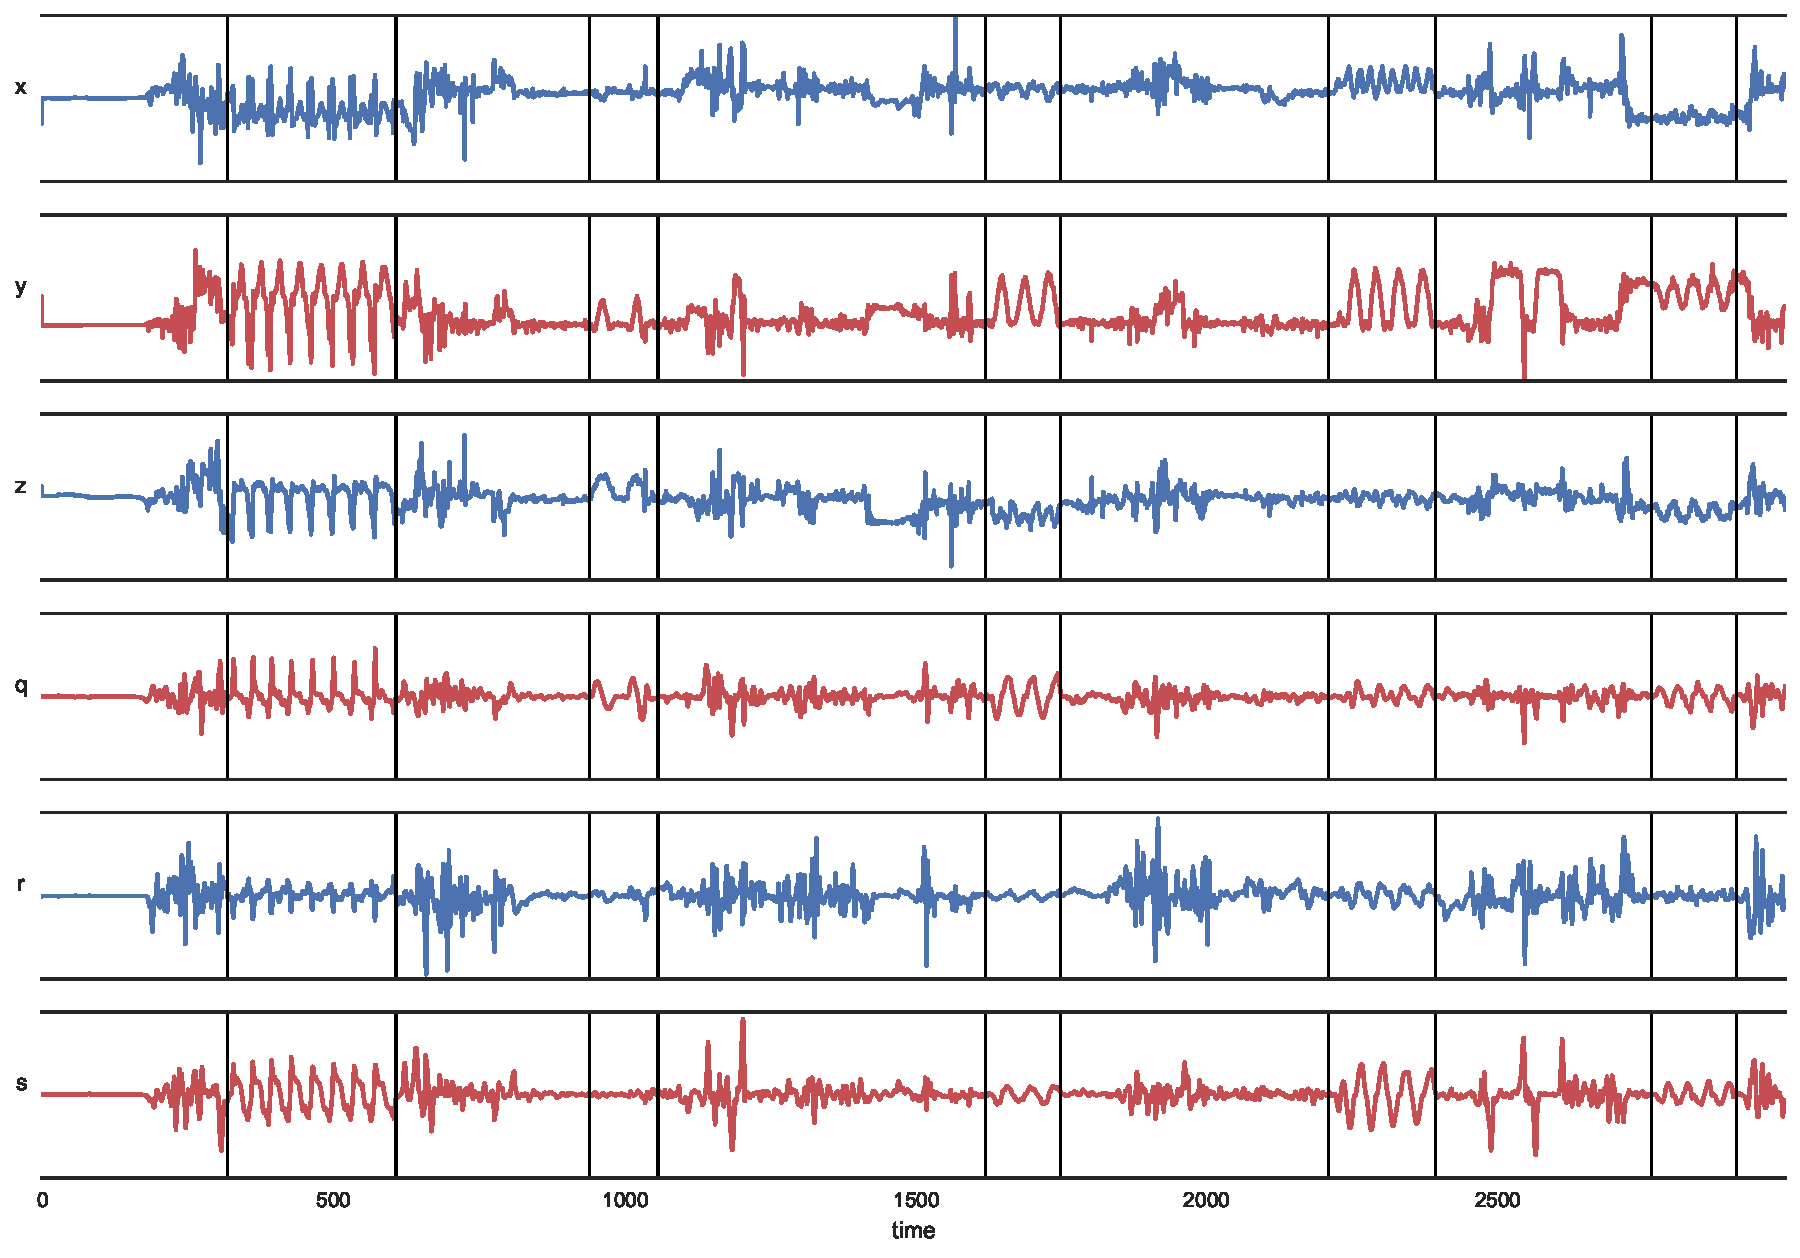
\includegraphics[width=1\textwidth]{img/routine_380.pdf}
    \caption[Example routine time series]{Example routine time series,
    vertically ordered by $x$, $y$, $z$ (accelerometer, axis range from -3 to 3)
    and $q$, $r$, $s$ (gyroscope, axis range from -600 to 600).}
    \label{fig:routine}
\end{figure}

\section{Exercise Taxonomy}
\label{sec:Exercise Taxonomy}
Exercise names are often ambiguous; several names can refer to the same exercise,
and the same name can refer to different variations of the same exercise.
The first type of naming ambiguity (many to one) is easily solved by defining a fixed reference name
which is always used, but the second type (one to many) is more difficult to handle.
\\\\
The second type of ambiguity typically involves positioning, resulting in exercises that are visually similar
but whose sensor readings can be drastically different.
Examples include supinated (underhand) vs pronated (overhand) for pull-ups and dumbbell curls,
or hands on temple vs hands behind head vs arms crossed for sit-ups and crunches. To solve this problem
a standard naming convention for exercises which include form variations was defined. This allows grouping
form variations into different classes, which was found to be beneficial for some classifiers.
The final naming convention we adopted is
\[
    \m{[modifier] [equipment] <exercise> [(form variation)]}
\]
where square brackets and angle brackets denote optional and required arguments respectively.
This convention results in exercise names such as
\[
    \underbrace{\text{alternating}}_{\text{modifier}} \; \underbrace{\text{dumbbell}}_{\text{equipment}} \; \underbrace{\text{bicep curl}}_{\text{exercise}} \; \underbrace{\text{(start with wrist facing forward)}}_{\text{form variation}}
\]
and
\[
    \underbrace{}_{\text{modifier}} \; \underbrace{}_{\text{equipment}} \; \underbrace{\text{pull-up}}_{\text{exercise}} \; \underbrace{\text{(supinated)}}_{\text{form variation}}
\]

\chapter{Hidden Markov Models}
\label{chap: Hidden Markov Models}
\acp{HMM}~\cite{rabiner-hmms} are a common theme throughout this thesis.
In the spirit of self containment this chapter introduces common terminology,
methods and inference algorithms employed when working with \acp{HMM}. In particular
the focus is on Bayesian methods. For a more standard introduction see Kevin Murphy's
excellent thesis~\cite{murphy-thesis}, which also discusses the more general class of probabilistic models
known as \acp{DBN}, of which \acp{HMM} and the popular Kalman filter~\cite{kalman-filter}, are a member.

\section{Introduction to Hidden Markov Models}
\label{sec:Introduction to Hidden Markov Models}
\acp{HMM} are probabilistic state-space models for sequential data.
The states in an \ac{HMM} are members of a finite discrete set, and
can be partitioned into a set of observed variables $X$, and latent
(unobserved) variables $Y$. The latent variables evolve according to
a first order Markov process:

\[
    P(y_t \mid \seq{y}{1}{t-1}) = P(y_t \mid y_{t-1})
\]

i.e., the latent state at time $t$ depends only on the latent state
at time $t-1$. Generalization to higher order dependencies is straightforward.
It is typically assumed that the observation at time $t$ is conditionally
independent of all other variables given the latent variable at time $t$,

\[
    P(x_t \mid \seq{y}{1}{T}) = P(x_t \mid y_t).
\]

Again, this assumption can be relaxed in obvious ways~\cite{autoregressive-shannon}.
For ease of exposition the simplest formulation presented above is used here.
\\\\
Given the above assumptions the joint probability of a sequence of observations
$\seq{x}{1}{T}$ and latent states $\seq{y}{1}{T}$ is given by

\begin{equation}\label{eq:hmm-joint}
    P(\seq{x}{1}{T}, \seq{y}{1}{T}) =
    P(y_1)P(x_1 \mid y_1) \prod_{t=2}^T P(y_t \mid y_{t-1}) P(x_t \mid y_t).
\end{equation}

The corresponding generative story is given by

\begin{enumerate}
    \item Sample an initial state $y_1 \sim \Cat(\pi_0)$.
    \item Sample an initial observation $x_t \sim \SomeDist(\phi_{y_1})$.
    \item For $t = 2$ to $T$
    \begin{enumerate}
        \item Sample the next state $y_{t} \mid z_t \sim \Cat(\pi_{y_{t-1}})$ conditioned on the previous state.
        \item Sample the next observation $x_t \mid y_t \sim \SomeDist(\phi_{y_t})$ conditioned on the current state.
    \end{enumerate}
\end{enumerate}

where $\SomeDist$ is some parametric emission distribution.
Dependencies can be visualized graphically in Figure~\ref{fig:hmm},
where vertices represent variables, edges represent dependencies,
and grey vertices represent observed variables.

\begin{figure}[ht!]
    \centering
    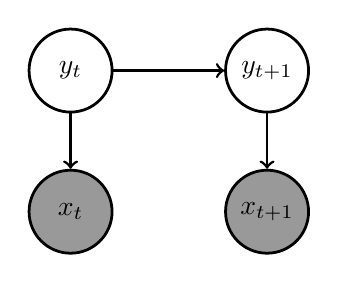
\begin{tikzpicture}
        \node[randvar] (y_t) {$y_t$};
        \node[randvar,fill=grey3,below=20pt of y_t] (x_t) {$x_t$};

        \node[randvar,right=40pt of y_t] (y_tp1) {$y_{t+1}$};
        \node[randvar,fill=grey3,below=20pt of y_tp1] (x_tp1) {$x_{t+1}$};

        \draw[->,line width=1pt] (y_t) to (y_tp1);
        \draw[->,line width=1pt] (y_t) to (x_t);
        \draw[->,line width=1pt] (y_tp1) to (x_tp1);
    \end{tikzpicture}
    \caption[Slice representation of a HMM]{
        Slice representation of a HMM.
        Conditional dependencies and random variables are denoted by
        directed edges and vertices respectively. Shaded vertices correspond
        to random variables which are be observed.
    }
    \label{fig:hmm}
\end{figure}

\subsection{Inference}
This Section outlines two useful algorithms for \acp{HMM}
assuming a fixed set of parameters. The first computes the
likelihood of an observed sequence under the given parameters.
The second computes the most likely sequence of states given
an observed sequence. The number of states in the \ac{HMM} will
be denoted by $K$.

\subsubsection{Likelihood}
Computing the likelihood of an observed sequence $\seq{x}{1}{T}$ can be done naively
by marginalizing over all possible length $T$ states sequences

\[
    P(\seq{x}{1}{T}) = \sum_{\seq{y}{1}{T}} P(\seq{x}{1}{T}, \seq{y}{1}{T})
\]

Computation in this manner requires time $O(TK^T)$ and is infeasible for all
but the smallest $K$ and $T$. A more efficient algorithm exists requiring only time
$O(TK^2)$. It is typically referred to as the forward, alpha, or
simply sum-product algorithm in the more general context of \acp{PGM}.
\\\\
Define $\alpha_{t,y_t} = P(y_t, \seq{x}{1}{t})$ as the joint probability
of the state at time $t$ being $y_t$ and the entire observation sequence up to
time $t$. The key insight is that $\alpha_{t,*}$ may be computed recursively
from $\alpha_{t-1,*}$ as

\begin{align*}
    \alpha_{t,y_t}
    &= P(y_t, \seq{x}{1}{t}) \\
    &= P(x_t \mid y_t) \sum_{y_{t-1}} P(y_t \mid y_{t-1}) P(y_{t-1}, \seq{x}{1}{t-1}) \\
    &= P(x_t \mid y_t) \sum_{y_{t-1}} P(y_t \mid y_{t-1}) \alpha_{t-1,y_{t-1}} \\
\intertext{with the base case given by}
    \alpha_{1,y_1} &= P(y_1)P(x_1 \mid y_1)\\
\end{align*}

It follows that

\[
    P(\seq{x}{1}{T}) = \sum_{y_T} P(y_T, \seq{x}{1}{T}) = \sum_{y_T} \alpha_{T,y_T}.
\]

\subsubsection{The Maximum a Posteriori State Sequence}
The algorithm for efficiently computing the most likely state sequence given an
observed sequence is closely related to the algorithm for computing the likelihood
of an observed sequence discussed above.
It is commonly referred to as the Viterbi or max-product algorithm.
\\\\
Define

\[
    v_{t,i} = \max_{\seq{y}{1}{t}}\{P(\seq{x}{1}{t}, \seq{y}{1}{t}) \mid y_t = i\}
\]

as the probability of the most likely sequence of $t$ states ending in state $i$
given $\seq{x}{1}{t}$. Then $v_{t,*}$ may be computed recursively from $v_{t-1,*}$ as

\begin{align*}
    v_{t,y_t}
    &= \max_{y_{t-1}}\{ P(x_{t} \mid y_t) P(y_t \mid y_{t-1}) v_{t-1,y_{t-1}} \} \\
    &= P(x_t \mid y_t) \max_{y_{t-1}}\{ P(y_t \mid y_{t-1}) v_{t-1,y_{t-1}} \} \\
\intertext{with the base case given by}
    v_{1,y_1} &= P(y_1)P(x_1 \mid y_1).
\end{align*}

The most likely path is easily recovered by storing a $T \times K$ table of back pointers
whose $t,k$ entry is the most likely state leading to state $k$ at time $t$.

\section{The Bayesian Approach}
Bayesian statistics treats quantities of interest as random variables.
In the context of Machine Learning, Bayesian methods are frequently used
for parameter estimation and model selection, although only the former is
considered here. The Bayesian approach to parameter estimation begins by
defining a prior distribution over model parameters before observing any data,
$P(\theta)$. After observing data $D$ one is typically interested in the
posterior, i.e., the probability distribution over parameters, conditioned on observing
$D$.

\[
    P(\theta \mid D) = \frac{P(\theta)P(D \mid \theta)}{P(D)}.
\]

The term $P(D \mid \theta)$ appearing above is referred to as the likelihood.
Using this terminology one is able to write
\[
    \text{Posterior} \propto \text{Prior} \times \text{Likelihood}.
\]

\subsection{The Dirichlet-Categorical Distribution}
The Dirichlet distribution is a probability distribution defined on the $K-1$
dimensional simplex $\triangle$. $\pi \in \triangle \implies \pi_k > 0$, $\sum_k \pi_k = 1$.
It is useful to conceptualize the Dirichlet distribution as a distribution over
parameters of Categorical or Multinomial distributions. From this point of view
samples from a Dirichlet distribution are themselves probability distributions.
\\\\
If $\pi \sim \Dir(\alpha)$ then

\begin{equation}
    P(\pi) = \frac{1}{\Bf(\alpha)} \prod_k \pi_k^{\alpha_k-1}, \label{eq:dir-pdf}
\end{equation}

where $\Bf$ is the multivariate beta function,

\begin{equation}
    \Bf(\alpha) = \frac{\prod_k \Gamma(\alpha_k)}{\Gamma(\sum_k \alpha_k)}, \label{eq:betafunc}
\end{equation}

and $\Gamma$ is the Gamma function.
\\\\
Let $D = \{x_1, \ldots, x_m\}$ and $n_k = \sum_{x \in D} \1\{x = k\}$ count
the number of occurrences of $k \in D$. Assuming

\begin{align*}
    \pi & \sim \Dir(\alpha) \\
    x_i & \sim \Cat(\pi),\; i = 1, \ldots, m.
\end{align*}

Then

\begin{align*}
    P(\pi \mid D, \alpha)
    &= \frac{P(\pi \mid \alpha) P(D \mid \pi, \alpha)}{P(D)} \\
    & \propto P(\pi \mid \alpha) P(D \mid \pi) \\
    &= \frac{1}{\Bf(\alpha)} \prod_k \pi_k^{\alpha_k - 1} \prod_k \pi_k^{n_k} \\
    &= \frac{1}{\Bf(\alpha)} \prod_k \pi_k^{n_k + \alpha_k - 1},
\end{align*}

The Dirichlet distribution is referred to as the \emph{conjugate} prior for the
Categorical distribution since the posterior $P(\pi \mid D, \alpha)$ and prior $P(\pi \mid \alpha)$
have the same form~\cite{gelman-bayesian-data-analysis}. The marginal likelihood $P(D \mid \alpha)$
can be obtained by integrating over $\pi$ as follows.

\begin{align}
    P(D \mid \alpha)
    &= \int_{\triangle} P(\pi \mid \alpha)\prod_{x \in D} P(x \mid \pi) d \pi \nonumber \\
    %
    &= \int_{\triangle} \frac{\Gamma(\sum_k \alpha_k)}{\prod_k \Gamma(\alpha_k)}
                        \prod_k \pi^{\alpha_k - 1}_k \prod_k \pi_k^{n_k} d \pi \nonumber \\
    %
    &= \frac{1}{\Bf(\alpha)}
       \int_{\triangle} \prod_k \pi_k^{n_k + \alpha_k - 1} d \pi. \label{eq:unnormed-dir}
\end{align}

The term inside the integral in (\ref{eq:unnormed-dir}) is the unnormalized \ac{pdf}
of a Dirichlet distribution with parameters $n_k + \alpha_k$. Since (\ref{eq:dir-pdf})
is a \ac{pdf} it follows that

\begin{align}
    1
    &= \int_\triangle \frac{1}{\Bf(\bm{n} + \alpha)} \prod_k \pi_k^{n_k + \alpha_k - 1} d \pi \nonumber \\
    &= \frac{1}{\Bf(\bm{n} + \alpha)} \int_\triangle \prod_k \pi_k^{n_k + \alpha_k - 1} d \pi \nonumber  \\
\implies \Bf(\bm{n} + \alpha) &= \int_\triangle \prod_k \pi_k^{n_k + \alpha - 1} d \pi \label{eq:dir-int-sol}
\end{align}

where $\bm{n} = (n_1, \ldots, n_K)$ is the vector of counts defined above.
Plugging (\ref{eq:dir-int-sol}) into (\ref{eq:unnormed-dir}) yields

\begin{equation}
    P(D \mid \alpha)
    = \frac{1}{\Bf(\alpha)}\int_{\triangle} \prod_k \pi_k^{n_k + \alpha_k - 1} d \pi
    = \frac{\Bf(\bm{n} + \alpha)}{\Bf(\alpha)}. \label{eq:dpcmarg}
\end{equation}

The process of marginalizing over a parameter as above is common in Bayesian analysis.
It is particularly helpful in the context of Gibbs sampling since reducing the number
of parameters that need to be sampled frequently results in increased efficiency.

\subsection{The Bayesian Hidden Markov Model}
Since the initial and transition distributions of an \ac{HMM} are Categorical distributions
it is convenient, due to the above described conjugacy relation, to place Dirichlet priors
with parameters $\alpha_0$ and $\alpha_i$ over their parameters $\pi_0$ and $\pi_i$.
Assuming each state's emission distribution is also Categorical
with parameters $\theta_i$, a Dirichlet prior with parameters $\alpha_i^\p$ may be placed
over these parameters as well. This results in the following generative story.

\begin{align*}
    \pi_0 & \sim \Dir(\alpha_0) \\
    \pi_i & \sim \Dir(\alpha_i),\; i = 1, \ldots, \abs{Y} \\
    \theta_i & \sim \Dir(\alpha_i^\p),\; i = 1, \ldots, \abs{Y} \\
    y_1 & \sim \Cat(\pi_0) \\
    y_{t+1} \mid y_t & \sim \Cat(\pi_{y_t}),\; t = 1, \ldots, T-1 \\
    x_t \mid y_t & \sim \Cat(\theta_{y_t}), \; t = 1, \ldots, T.
\end{align*}

Let $(\mathcal{X}, \mathcal{Y}) = (\{\seq{x}{1}{T_1}^1, \ldots, \seq{x}{1}{T_m}^m\},
\{\seq{y}{1}{T_1}^1, \ldots, \seq{y}{1}{T_m}^m\})$ be a set of
observation and corresponding state sequences, and

\begin{align*}
    n_{0, i} &= \sum_{y \in \mathbf{y}} \1\{y_1 = i\} \\
    n_{i, j} &= \sum_{y \in \mathbf{y}} \sum_{t} \1\{y_{t-1} = i \wedge y_t = j\} \\
    n_{i, o}^\p &= \sum_{(\seq{x}{1}{T},\seq{y}{1}{T}) \in (\mathcal{X},\mathcal{Y})} \sum_{t} \1\{y_t = i \wedge x_t = o\} \\
\end{align*}

count the number of times the initial states is $i$, the number of transition from state $i$ to $j$,
and the number of times a particular observation $o$ is observed in state $i$ respectively. Then

\begin{align}  \label{eq:bayes-hmm-joint-simple}
 P(\mathcal{X}, \mathcal{Y} \mid \Theta, \alpha)
 &=  P(\pi_0 \mid \alpha_0) \prod_i P(\pi_i \mid \alpha_i) \prod_i P(\theta_i \mid \alpha^\prime) \nonumber\\
 & \times \prod_{(\seq{x}{1}{T},\seq{y}{1}{T}) \in (\mathcal{X},\mathcal{Y})} P(\seq{x}{1}{T},\seq{y}{1}{T})
\end{align}

where $\Theta = \{\pi_0, \pi_i, \theta_i\}$ and $\alpha = \{\alpha_0, \alpha_i, \alpha_i^\prime\}$.
\\\\
Substituting the equations for the of the priors into (\ref{eq:bayes-hmm-joint-simple})
and rewriting in terms of the counting variables gives,

\begin{align} \label{eq:bayes-hmm-joint-full}
    P(\mathcal{X}, \mathcal{Y} \mid \Theta, \alpha)
    &= \frac{1}{\Bf(\alpha_0)} \prod_{i} \pi_{0,i}^{n_{0,i} + \alpha_{0,i} - 1} \nonumber \\
    & \times \prod_i \left(\frac{1}{\Bf(\alpha_i)} \prod_{j} \pi_{i,j}^{n_{i,j} + \alpha_{i,j} - 1}\right) \nonumber \\
    & \times \prod_i \left(\frac{1}{\Bf(\alpha_i^\prime)} \prod_{v} \pi_{i,j}^{n_{i,v}^\prime + \alpha_{i,v}^\prime - 1}\right).
\end{align}

Repeatedly applying the same steps used to derive (\ref{eq:dir-int-sol})
allows one to write the marginal joint probability of $(\mathcal{X}, \mathcal{Y})$
in terms of hyperparameters and counts.

\begin{equation}
    P(\mathcal{X}, \mathcal{Y} \mid \alpha_0, \alpha_i, \alpha_i^\prime)
    = \frac{\Bf((\bm{n}_0 + \alpha_0)}{\Bf(\alpha_0)}
    \prod_i \frac{\Bf{(\bm{n}_i + \alpha_i}}{\Bf(\alpha_i)}
    \frac{\Bf((\bm{n}_i^\p + \alpha_i^\p)}{\Bf(\alpha_i^\p)}
    \label{eq:marg-likelihood-hmm}
\end{equation}

where the counts have been extended to vectors as was done previously,

\begin{align*}
    \bm{n}_0 &= (n_{0,1}, \ldots, n_{0,\abs{Y}}) \\
    \bm{n}_i &= (n_{i,1}, \ldots, n_{i,\abs{Y}}),\; i = 1, \ldots, \abs{Y} \\
    \bm{n}_i^\p &= (n_{i,1}^\p, \ldots, n_{i,\abs{X}}^\p),\; i = 1, \ldots, \abs{Y}. \\
\end{align*}

From an algorithmic perspective (\ref{eq:marg-likelihood-hmm}) has a particularly convenient
form. Given the counting variables the time required to compute the marginal likelihood does not
depend on the number of sequences or their length, only the number of states and and possible observations.

\section{A Block Collapsed Gibbs Sampler for Hidden Markov Models}
\label{sec:A Block Collapsed Gibbs Sampler for Hidden Markov Models}
This Section develops a collapsed Gibbs Sampler for $P(\mathcal{Y} \mid \mathcal{X}, \alpha)$.
We do so using a block-wise approach, resampling an entire state sequence $\seq{y}{1}{T}^i$ given
$\mathcal{X}$, $\mathcal{Y}_{-i}, \alpha$, where $\mathcal{Y}_{-i}$ denotes
$\mathcal{Y} \setminus \{\seq{y}{1}{T}^i\}$. This sampler follows the approach
described in~\cite{pcfg-bayesian-johnson} for \acp{PCFG}, and utilized
for \acp{HMM} in~\cite{hmm-comparison-johnson}.
\\\\
\begin{figure}[ht!]
    \centering
    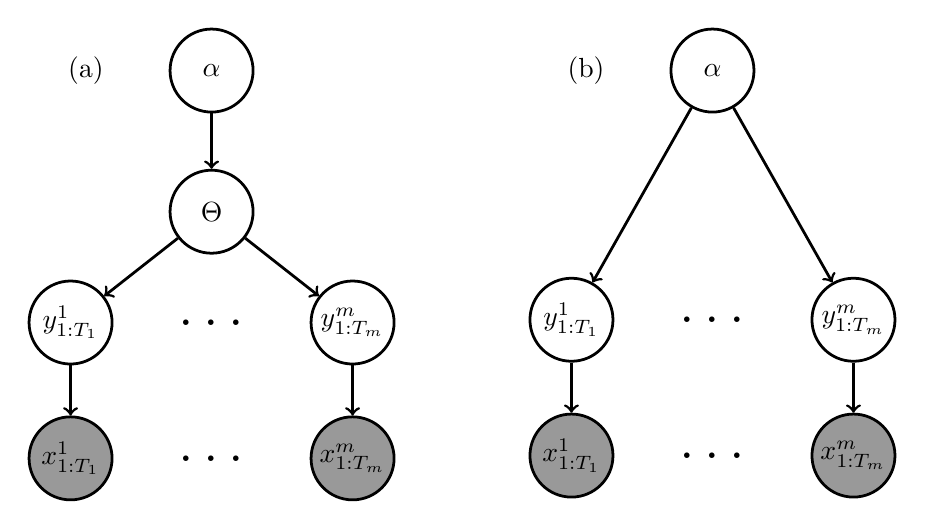
\begin{tikzpicture}
        \node[randvar] (alpha) {$\alpha$};
        \node[textbox,left=20pt of alpha] (a) {\normalsize{(a)}};
        \node[randvar,below=20pt of alpha] (Theta) {$\Theta$};
        \node[textbox,below=20pt of Theta] (ydots) {\huge{$\ldots$}};
        \node[randvar,left=20pt of ydots] (y1) {$\seq{y}{1}{T_1}^1$};
        \node[randvar,right=20pt of ydots] (ym) {$\seq{y}{1}{T_m}^m$};
        \node[textbox,below=40pt of ydots] (xdots) {\huge{$\ldots$}};
        \node[randvar,fill=grey3,left=20pt of xdots] (x1) {$\seq{x}{1}{T_1}^1$};
        \node[randvar,fill=grey3,right=20pt of xdots] (xm) {$\seq{x}{1}{T_m}^m$};

        \node[randvar,right=150pt of alpha] (alpha-marg) {$\alpha$};
        \node[textbox,left=20pt of alpha-marg] (b) {\normalsize{(b)}};
        \node[textbox,below=70pt of alpha-marg] (ydots-marg) {\huge{$\ldots$}};
        \node[randvar,left=20pt of ydots-marg] (y1-marg) {$\seq{y}{1}{T_1}^1$};
        \node[randvar,right=20pt of ydots-marg] (ym-marg) {$\seq{y}{1}{T_m}^m$};
        \node[textbox,below=40pt of ydots-marg] (xdots-marg) {\huge{$\ldots$}};
        \node[randvar,fill=grey3,left=20pt of xdots-marg] (x1-marg) {$\seq{x}{1}{T_1}^1$};
        \node[randvar,fill=grey3,right=20pt of xdots-marg] (xm-marg) {$\seq{x}{1}{T_m}^m$};

        \draw[->,line width=1pt] (alpha) to (Theta);
        \draw[->,line width=1pt] (Theta) to (y1);
        \draw[->,line width=1pt] (Theta) to (ym);
        \draw[->,line width=1pt] (y1) to (x1);
        \draw[->,line width=1pt] (ym) to (xm);

        \draw[->,line width=1pt] (alpha-marg) to (y1-marg);
        \draw[->,line width=1pt] (alpha-marg) to (ym-marg);
        \draw[->,line width=1pt] (y1-marg) to (x1-marg);
        \draw[->,line width=1pt] (ym-marg) to (xm-marg);
    \end{tikzpicture}
    \caption[Bayesian HMM with and without collapsing]{
        Graphical representation of a Bayesian HMM without (a) and with (b)
        marginalization of the parameters $\Theta$. Notice that marginalization
        of $\Theta$ introduces dependencies between latent states $y$, since
        they now share a common parent $\alpha$ in (b).
    }
    \label{fig:hmm-marg}
\end{figure}
The primary difficulty in constructing such a sampler is due to marginalizing over the parameters,
as doing so introduces dependencies among the latent state sequences $\mathcal{Y}$, Figure~\ref{fig:hmm-marg}.
Let us proceed in the usual manner for constructing such a Gibbs sampler. We have

\begin{equation}
    P(\seq{y}{1}{T}^i \mid \mathcal{Y}_{-i}, \mathcal{X}, \alpha)
    = \frac{P(\seq{x}{1}{T}^i \mid \seq{y}{1}{T}^i)P(\seq{y}{1}{T}^i \mid \mathcal{Y}_{-i}, \mathcal{X}_{-i}, \alpha)}
      {P(\seq{x}{1}{T}^i \mid \mathcal{Y}_{-i}, \mathcal{X}_{-i}, \alpha)}. \label{eq:hmm-gibbs-problem}
\end{equation}

The $P(\seq{x}{1}{T}^i \mid \mathcal{Y}_{-i}, \mathcal{X}_{-i}, \alpha)$ term in the denominator
of (\ref{eq:hmm-gibbs-problem}) is particularly problematic, as noted in~\cite{pcfg-bayesian-johnson}.
The need to marginalize over all possible state sequences (without reference to a set of \ac{HMM} parameters)
is particularly difficult, and it is not clear how one would approach such a problem
in a computationally efficient manner.
\\\\
Instead, since the denominator of (\ref{eq:hmm-gibbs-problem}) does not depend on $\seq{y}{1}{T}^i$,
we can appeal to a Metropolis-Hastings approach, knowing this troublesome term will cancel when
computing the acceptance probability.
\\\\
A Metropolis-Hastings sampler~\cite{mcmc-ml} is a popular \ac{MCMC} algorithm for drawing samples
from a target distribution $P(X)$, provided one is able to compute a value
$f(x)$ such that $f(x) \propto P(x)$. The sampler works by repeatedly drawing a
sample $x^*$ from a proposal distribution $q(\cdot \mid x)$ which is probabilistically
accepted, replacing the current $x$, or rejected. The result is a series of samples
whose stationary distribution is $P(X)$. In the special case that the proposal distribution
does not depend on the current sample, $q(x^* \mid x) = q(x^*)$, the proposal is said to
be \emph{independent}. The generic Metropolis-Hastings algorithm is given in Algorithm~\ref{alg:mh-generic}.

\begin{algorithm}[H]
    \caption{The Metropolis-Hastings Algorithm.\label{alg:mh-generic}}
    \begin{algorithmic}[1]
        \Require{$x^0$ starting value}
        \For{$i \gets 1, \ldots, n$}
            \State $x^* \sim q(\cdot \mid x^{i-1})$
            \State $u \sim \Unif(0, 1)$
            \If{$u < \dfrac{f(x^*) q(x^{i-1} \mid x^*)}{f(x^i) q(x^* \mid x^{i-1})}$}
                \State $x^i \gets x^*$
            \Else
                \State $x^i \gets x^{i-1}$
            \EndIf
        \EndFor
        \State \Return{$(x^1, \ldots, x^n)$}
    \end{algorithmic}
\end{algorithm}

For the problem of sampling a state sequence $\seq{y}{1}{T}$, the Metropolis-Hastings algorithm
is utilized as a subroutine to sample from the conditional distribution required
by the Gibbs sampler. This is known as Metropolis-within-Gibbs~\cite{mh-within-gibbs}.
Let $\mathcal{Y}^* = \{\seq{y}{1}{T}\}^* \cup \mathcal{Y}_{-i}$,
where $\seq{y}{1}{T}^*$ is drawn from some an independent distribution $q(\cdot)$.
Then the proposed $\seq{y}{1}{T}^*$ is accepted with probability
\begin{align}
    p
    &= \frac{P(\seq{y}{1}{T}^* \mid \mathcal{Y}_{-i}, \mathcal{X}, \alpha)}
            {P(\seq{y}{1}{T}^i \mid \mathcal{Y}_{-i}, \mathcal{X}, \alpha)} \
            \frac{q(\seq{y}{1}{T}^i)}{q(\seq{y}{1}{T}^*)} \nonumber \\
    &= \frac{P(\mathcal{Y}^*, \mathcal{X} \mid \alpha)}
            {P(\mathcal{Y}, \mathcal{X} \mid \alpha)}
            \frac{q(\seq{y}{1}{T}^i)}{q(\seq{y}{1}{T}^i*)} \nonumber \\
    &= \frac{\Bf(\bm{n}_0^* + \alpha_0)}
            {\Bf(\bm{n}_0 + \alpha_0)}
    \prod_j \left[ \frac{\Bf(\bm{n}_j^* + \alpha_j)}
                        {\Bf(\bm{n}_j + \alpha_j)}
                   \frac{\Bf(\bm{n}_j^{\prime *} + \alpha_j^\p)}
                        {\Bf(\bm{n}_j^\p + \alpha_j^\p)}\right]
                   \frac{q(\seq{y}{1}{T}^i)}{q(\seq{y}{1}{T}^*)} \label{eq:mh-hmm-prob-accept}
\end{align}

where the $\bm{n}^*$ are analogous to the $\bm{n}$ terms, but contain the
counts from the proposal $\seq{y}{1}{T}^*$ rather than $\seq{y}{1}{T}^i$.
\\\\
The proposal distribution $q(\cdot)$ is itself a \ac{HMM} with parameters
$\hat{\Theta} = \{\hat{\pi}_0, \hat{\pi}_i, \hat{\theta}_i\}$ derived from the current
$\mathcal{Y}_{-i}$, $\mathcal{X}_{-i}$. In particular $\hat{\Theta}$ is set to its expected value,
$\hat{\Theta} = \E[\Theta \mid Y_{-i}, X_{-i}, \alpha]$, and then the proposal is sampled from

\[
    \seq{y}{1}{T}^* \sim P(\cdot \mid \seq{x}{1}{T}^i, \hat{\Theta}).
\]
Empirically this strategy results in a majority of proposals $\seq{y}{1}{T}^*$ being accepted,
which aligns with the observations reported by~\cite{hmm-comparison-johnson}.
\\\\
To sample a latent state sequence the algorithm described in~\cite{scott-bayesian-hmm} is used.
The algorithm takes as input an observation sequence $\seq{x}{1}{T}$ and iteratively computes
$p_i^t = P(Y_t=i \mid \seq{x}{1}{t})$ from $P(y_{t-1} \mid \seq{x}{1}{t-1})$ in
a manner similar to the forward algorithm described in Section~\ref{sec:Introduction to Hidden Markov Models}.
However, along the way a series of matrices $A^t$ are computed such that
$a_{ij}^t = P(Y_{t-1}=i, Y_{t}=j, x_t \mid \seq{x}{1}{t-1})$. Once $p_i^T$
is computed the latent state sequence is sampled in reverse order starting by
sampling $y_T \sim \Cat(p^T)$. Having obtained a value for $y_t$, the algorithm
then samples $y_{t-1} \sim \Cat(b)$, where $b$ is proportional to the $y_t$ column
of $A^t$. A complete description is given in Algorithm~\ref{alg:sample-states}.

\begin{algorithm}[H]
    \caption{Sample States.\label{alg:sample-states}}
    \begin{algorithmic}[1]
        \Require{Observation sequence $\seq{x}{1}{T}$.}
        \Ensure{A sequence of laent state $\seq{y}{1}{T}$.}
        \State
        \State \(\triangleright\) Forward Traversal
        \State $u_j^1 \gets P(y_i)P(x_1 \mid y_i)$
        \State $p_j^1 \gets \dfrac{u_j^1}{\sum_i u_i^1}$
        \For{$t \gets 2, \ldots, T$}
            \State $u_{ij}^t \gets p_i^{t-1}P(j \mid i)P(x_t \mid j)$
            \State $a_{ij}^t \gets \dfrac{u_{ij}^t}{\sum_{i^\p j^\p} u_{i^\p j^\p}^t}$
            \State $p_j^t \gets \sum_i a_{ij}^t$
        \EndFor
        \State
        \State \(\triangleright\) Backward Sampling
        \State $y_T \sim \Cat(p^T)$
        \For{$t \gets T, \ldots, 2$}
            \State $b_i \gets \dfrac{a_{i y_t}^t}{\sum_{i^\p}a_{i^\p y_t}^t}$
            \State $y_{t-1} \sim \Cat(b)$
        \EndFor
        \State \Return $\seq{y}{1}{T}$
    \end{algorithmic}
\end{algorithm}


\section{Mixtures of Hidden Markov Models}
\label{sec:Mixtures of Hidden Markov Models}
Extension to a finite mixture of $K$ \acp{HMM} is straightforward and results
in the following generative story

\begin{align*}
    \phi & \sim \Dir(\beta) \\
    \pi_{k,0} & \sim \Dir(\alpha_0), k=1,\ldots,K \\
    \pi_{k,i} & \sim \Dir(\alpha_i),\; k=1,\ldots,K,\; i=1,\ldots,\abs{Y} \\
    \theta_{k,i} & \sim \Dir(\alpha_i^\p),\; k=1,\ldots,K,\; i = 1,\ldots,\abs{Y} \\
    z & \sim \Cat(\phi) \\
    \seq{x}{1}{T}, \seq{y}{1}{T} \mid z & \sim \HMM(\Theta_z).
\end{align*}

where $\HMM(\Theta_z)$ is used as shorthand for the \ac{HMM}
generative story outlined in Section~\ref{sec:Introduction to Hidden Markov Models}.
Again, the marginal likelihood $\mathcal{Z}$, $\mathcal{Y}$, and $\mathcal{X}$ can be
expressed in closed form in terms of hyper parameters and counts.

\begin{multline}
    P(\mathcal{Z}, \mathcal{X}, \mathcal{Y} \mid \alpha, \beta) = \\
    \frac{\Bf(\bm{c} + \beta)}{\Bf(\beta)}
    \prod_k
    \left(
        \frac{\Bf(\bm{n}_{k,0} + \alpha_0)}{\Bf(\alpha_0)}
        \prod_i
        \left(
            \frac{\Bf(\bm{n}_{k,i} + \alpha_i)}{\Bf(\alpha_i)}
            \frac{\Bf(\bm{n}_{k,i}^\p + \alpha_i^\p)}{\Bf(\alpha_i^\p)}
        \right)
    \right). \label{eq:joint-marg-finite-mixture}
\end{multline}

where $c_k = \sum_{z \in \mathcal{Z}}\1\{z = k\}$ and $\bm{c} = (c_1, \ldots, c_K)$.
\\\\
In many situations $K$ is unknown. Estimation of $K$ can be carried out using standard
techniques such as cross validation or Bayesian Information Criterion, but this is
often computationally difficult and methodologically unsatisfying. A modern
approach to dealing with this problem is Bayesian nonparametrics~\cite{jordan-bayesian-nonparam}.
In brief, Bayesian nonparametric techniques allow one to sidestep the problems associated with finite
capacity models, by assuming observations are generated from infinite dimensional objects,
for which only a finite number are involved in the generation of a finite set of samples.
\\\\
In the case of mixture models, the above model can naturally be extended to handle a
countably infinite number of cluster components using a Dirichlet Process~\cite{teh-dirichlet}.
The constructive definition of the Dirichlet process is given in terms of a
\emph{stick-breaking process}~\cite{sethuraman-constructive} with parameter
$\beta \in \mathbb{R}_{>0}$, frequently denoted $\GEM(\beta)$.

\begin{align*}
    \xi_k & \sim \Beta(1, \beta), k = 1,\ldots,\infty\\
    \phi_k & = \xi_k \prod_{l=1}^{k-1} (1 - \xi_l) \\
    \implies \phi & \sim \GEM(\beta) \\
\end{align*}

Extension of the finite mixture of \acp{HMM} to the nonparametric case thus assumes cluster
assignments are sampled from an infinite dimensional $\phi$, itself sampled
from a $\GEM(\beta)$ distribution.

\begin{align*}
    \phi & \sim \GEM(\beta) \\
    \pi_{k,0} & \sim \Dir(\alpha_0), k=1,\ldots,\infty \\
    \pi_{k,i} & \sim \Dir(\alpha_i),\; k=1,\ldots,\infty,\; i=1,\ldots,\abs{Y} \\
    \theta_{k,i} & \sim \Dir(\alpha_i^\p),\; k=1,\ldots,\infty,\; i = 1,\ldots,\abs{Y} \\
    z & \sim \phi \\
    \seq{x}{1}{T}, \seq{y}{1}{T} \mid z & \sim \HMM(\Theta_z).
\end{align*}

Note that for any finite set of $\{z_1, \ldots, z_m\} = \mathcal{Z}$,
$\bm{c}$ contains at most $m$ unique elements. In analogy to the finite
mixture model, denote the number of unique elements $K$. Then the marginal likelihood
of $\bm{c}$ given $\beta$ has the following form~\cite{kyung-estimation-dirichlet}

\begin{equation}\label{dp-marg}
    P(\bm{c} \mid \beta) = \frac{m^K \Gamma(\beta)}{\Gamma(\beta + m)} \prod_k \Gamma(c_k).
\end{equation}

Collapsing all parameters results in the following slight alteration of
equation ($\ref{eq:joint-marg-finite-mixture}$).

\begin{multline}
    P(\mathcal{Z}, \mathcal{X}, \mathcal{Y} \mid \alpha) =
    \left(\frac{m^K \Gamma(\beta)}{\Gamma(\beta + m)} \prod_k \Gamma(c_k)\right) \\
    \times \prod_k
    \left(
        \frac{\Bf(\bm{n}_{k,0} + \alpha_0)}{\Bf(\alpha_0)}
        \prod_i
        \left(
            \frac{\Bf(\bm{n}_{k,i} + \alpha_i)}{\Bf(\alpha_i)}
            \frac{\Bf(\bm{n}_{k,i}^\p + \alpha_i^\p)}{\Bf(\alpha_i^\p)}
        \right)
    \right). \label{eq:joint-marg-infinite-mixture}
\end{multline}

Having derived an expression for the the marginal likelihood of an infinite
mixture of \acp{HMM}, the same generic Metropolis-within-Gibbs approach presented
in Section~\ref{sec:A Block Collapsed Gibbs Sampler for Hidden Markov Models}
could be applied to carry out inference in the infinite mixture of \acp{HMM}.
\\\\
However, collapsed Gibbs sampling for Dirichlet processes is a well studied problem for
which numerous solutions exist~\cite{neal-mcmc-dp}. In particular it would be easy
to alternate between sampling $z_i$ variables and latent state sequences $\seq{y}{1}{T}^i$.
Unfortunately this would likely mix poorly, since the sequence of latent states should be highly
dependent on the cluster assignment. The ability to propose a new cluster and a new state sequence
simultaneously avoids this problem, motivating the desire to blockwise sample
in the combined space $(z_i, y^i_1, y^i_2, \ldots, y^i_T)$.
\\\\
Luckily the marginal posterior predictive distribution of a Dirichlet process has a particularly
convenient form~\cite{infinite-gmm} given by
\[
    P(z_i=k|\mathcal{Z}_{-i}) \propto
    \begin{cases}
        c_{k,-i} & k \in \mathcal{Z}_{-i} \\
        \beta   & k \not\in \mathcal{Z}_{-i}.
    \end{cases}
\]
Unlike proposing a latent state sequence, proposing $z_i$ from this distribution is straightforward.
Incorporating this into the proposal distribution means the terms related to the Dirichlet Process
will cancel, and can be neglected when calculating the acceptance ratio of the Metropolis within Gibbs sampler.


\chapter{A Generative Model for Repetitive Sequences}
\label{chap: A Generative Model for Repetitive Sequences}
A significant advantage of \acp{PGM} over popular discriminative Machine Learning methods
such as \acp{SVM}, Random Forests, or Neural Networks, is the ability to easily incorporate
structured knowledge via latent variables and conditional dependencies into the
models~\cite{structured-priors,poverty-stimulus,how-to-grow-a-mind}.
This is true even in the case when the structure itself is unobserved, and must
be learned in an unsupervised manner. This chapter describes a structured generative model for
repetitive sequences. The model is a \ac{HMM} with cyclically structured transitions which,
for brevity, will be dubbed the \ac{CHMM}.
\\\\
This model is specifically designed to reflect the structure of the repetitive sequences
often encountered in activity recognition. While there have been several previous studies demonstrating
the effectiveness of \acp{HMM} for recognizing activities from wearable sensors~\cite{hhmm-lee,factored-hmm-tran},
to date none have explicitly designed models to account for the repetitive nature
of many activities. Repetition is a powerful inductive bias that can easily be incorporated into
\ac{DBN} models (such as \acp{HMM}). This is especially relevant in the exercise recognition
domain as all activities considered are repetitive.
\\\\
Using \ac{HMM}s with structured transitions to model specific properties of sequences is
not entirely novel. \cite{cascaded-finite-state} use a similarly structured model to develop
a high accuracy unsupervised grammar induction system.

\section{Motivation}
The structure of the model used is motivated by the observation that artificial
sequences which resemble sensor reading during an exercise can be recognized by a \ac{DFA}
with cyclic transition structures. Consider the oscillatory discrete time series depicted
in Figure~\ref{fig:osc-step}.

\begin{figure}[H]
    \centering
    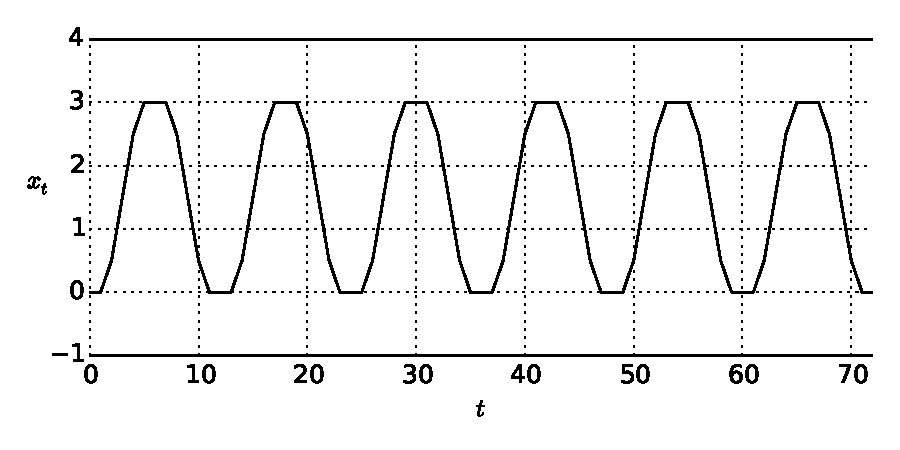
\includegraphics[width=1\textwidth]{img/osc-step.pdf}
    \caption[Oscillatory discrete time series]{
        Example of a synthetic oscillatory discrete time series.
    }
    \label{fig:osc-step}
\end{figure}

Taking the difference between successive values $x_t$ and $x_{t+1}$
as symbols in an alphabet, this sequence belongs to the regular language

\[
    \left[
        \left[+0\right]^*
        \left[+\tfrac{1}{2}\right]^+
        \left[+1\right]^*
        \left[+\tfrac{1}{2}\right]^+
        \left[+0\right]^*
        \left[-\tfrac{1}{2}\right]^+
        \left[-1\right]^*
        \left[-\tfrac{1}{2}\right]^+
    \right]^*,
\]

which is recognized by the \ac{DFA} in Figure~\ref{fig:cyclic-dfa}.

\begin{figure}[H]
    \centering
    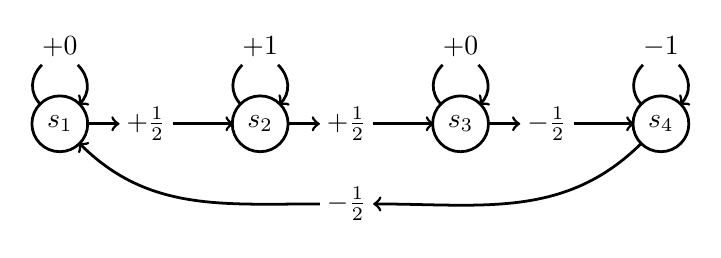
\begin{tikzpicture}
        \tikzstyle{every circle node}=[circle,draw,minimum size=20pt,line width=1pt];
        \node[circle] (s1) {$s_1$};
        \node[textbox,font=\normalsize,above=10pt of s1] (s1s1) {$+0$};
        \node[textbox,font=\normalsize,right=10pt of s1] (s1s2) {$+\frac{1}{2}$};

        \node[circle,right=20pt of s1s2] (s2) {$s_2$};
        \node[textbox,font=\normalsize,above=10pt of s2] (s2s2) {$+1$};
        \node[textbox,font=\normalsize,right=10pt of s2] (s2s3) {$+\frac{1}{2}$};

        \node[circle,right=20pt of s2s3] (s3) {$s_3$};
        \node[textbox,font=\normalsize,above=10pt of s3] (s3s3) {$+0$};
        \node[textbox,font=\normalsize,right=10pt of s3] (s3s4) {$-\frac{1}{2}$};

        \node[circle,right=20pt of s3s4] (s4) {$s_4$};
        \node[textbox,font=\normalsize,above=10pt of s4] (s4s4) {$-1$};
        \node[textbox,font=\normalsize,below=10pt of s2s3] (s4s1) {$-\frac{1}{2}$};

        \draw[line width=1pt,shorten >= -1pt, shorten <= -1pt] (s1) to[in=225,out=135] (s1s1);
        \draw[->,line width=1pt,shorten >= -1pt, shorten <= -1pt] (s1s1) to[in=45,out=315] (s1);
        \draw[->,line width=1pt,shorten >= -1pt, shorten <= -1pt] (s1) to (s1s2);
        \draw[->,line width=1pt,shorten >= -1pt, shorten <= -1pt] (s1s2) to (s2);

        \draw[line width=1pt,shorten >= -1pt, shorten <= -1pt] (s2) to[in=225,out=135] (s2s2);
        \draw[->,line width=1pt,shorten >= -1pt, shorten <= -1pt] (s2s2) to[in=45,out=315] (s2);
        \draw[->,line width=1pt,shorten >= -1pt, shorten <= -1pt] (s2) to (s2s3);
        \draw[->,line width=1pt,shorten >= -1pt, shorten <= -1pt] (s2s3) to (s3);

        \draw[line width=1pt,shorten >= -1pt, shorten <= -1pt] (s3) to[in=225,out=135] (s3s3);
        \draw[->,line width=1pt,shorten >= -1pt, shorten <= -1pt] (s3s3) to[in=45,out=315] (s3);
        \draw[->,line width=1pt,shorten >= -1pt, shorten <= -1pt] (s3) to (s3s4);
        \draw[->,line width=1pt,shorten >= -1pt, shorten <= -1pt] (s3s4) to (s4);

        \draw[line width=1pt,shorten >= -1pt, shorten <= -1pt] (s4) to[in=225,out=135] (s4s4);
        \draw[->,line width=1pt,shorten >= -1pt, shorten <= -1pt] (s4s4) to[in=45,out=315] (s4);
        \draw[->,line width=1pt,shorten >= -1pt, shorten <= -1pt] (s4) to[in=0,out=225] (s4s1);
        \draw[->,line width=1pt,shorten >= -1pt, shorten <= -1pt] (s4s1) to[in=315,out=180] (s1);
    \end{tikzpicture}
    \caption[Cyclic DFA]{
        Cyclic DFA with four states.
    }
    \label{fig:cyclic-dfa}
\end{figure}

The natural probabilistic generalization of this \ac{DFA} is a \ac{HMM}
with a cyclic transition structure and parametric emission distributions replacing
discrete symbols, Figure~\ref{fig:cyclic-hmm}.

\begin{figure}[H]
    \begin{tikzpicture}
        \tikzstyle{every circle node}=[circle,draw,minimum size=20pt,line width=1pt];
        \node[circle] (s1) {$s_1$};
        \node[textbox,below=20pt of s1] (e1) {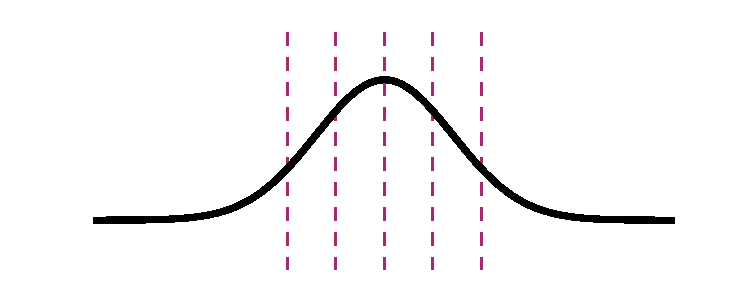
\includegraphics[width=0.25\textwidth]{img/gauss/gauss-0.pdf}};
        \node[textbox,font=\normalsize,above=20pt of s1] (s1s1) {$P(s_1|s_1)$};
        \node[textbox,font=\normalsize,right=10pt of s1] (s1s2) {$P(s_2|s_1)$};

        \node[circle,right=10pt of s1s2] (s2) {$s_2$};
        \node[textbox,below=20pt of s2] (e2) {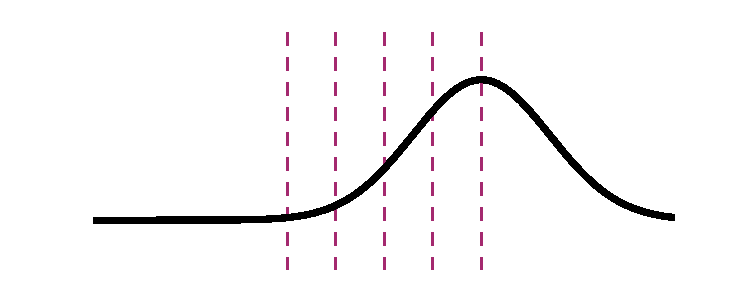
\includegraphics[width=0.25\textwidth]{./img/gauss/gauss-1.pdf}};
        \node[textbox,font=\normalsize,above=20pt of s2] (s2s2) {$P(s_2|s_2)$};
        \node[textbox,font=\normalsize,right=10pt of s2] (s2s3) {$P(s_3|s_2)$};

        \node[circle,right=10pt of s2s3] (s3) {$s_3$};
        \node[textbox,below=20pt of s3] (e3) {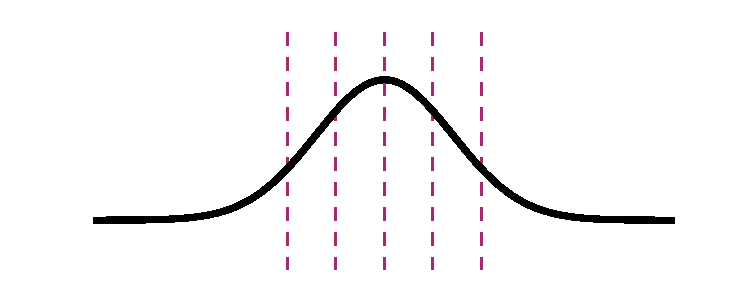
\includegraphics[width=0.25\textwidth]{./img/gauss/gauss-0.pdf}};
        \node[textbox,font=\normalsize,above=20pt of s3] (s3s3) {$P(s_3|s_3)$};
        \node[textbox,font=\normalsize,right=10pt of s3] (s3s4) {$P(s_4|s_3)$};

        \node[circle,right=10pt of s3s4] (s4) {$s_4$};
        \node[textbox,below=20pt of s4] (e4) {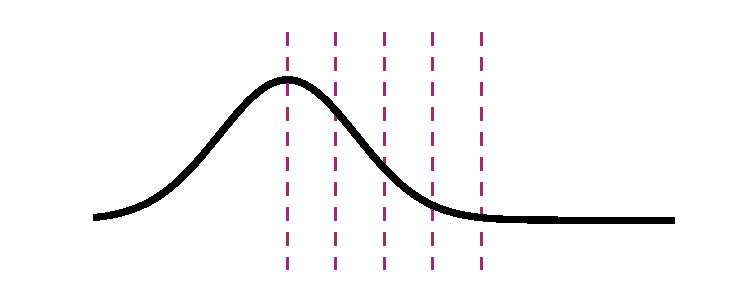
\includegraphics[width=0.25\textwidth]{./img/gauss/gauss-neg1.pdf}};
        \node[textbox,font=\normalsize,above=20pt of s4] (s4s4) {$P(s_4|s_4)$};
        \node[textbox,font=\normalsize,above=40pt of s2s3] (s4s1) {$P(s_1|s_4)$};

        \draw[line width=1pt,shorten >= -1pt, shorten <= -1pt] (s1) to[in=225,out=135] (s1s1);
        \draw[->,line width=1pt,shorten >= -1pt, shorten <= -1pt] (s1s1) to[in=45,out=315] (s1);
        \draw[->,line width=1pt,shorten >= -1pt, shorten <= -1pt] (s1) to (s1s2);
        \draw[->,line width=1pt,shorten >= -1pt, shorten <= -1pt] (s1s2) to (s2);
        \draw[->,line width=1pt,shorten >= -1pt, shorten <= -1pt] (s1) to (e1);

        \draw[line width=1pt,shorten >= -1pt, shorten <= -1pt] (s2) to[in=225,out=135] (s2s2);
        \draw[->,line width=1pt,shorten >= -1pt, shorten <= -1pt] (s2s2) to[in=45,out=315] (s2);
        \draw[->,line width=1pt,shorten >= -1pt, shorten <= -1pt] (s2) to (s2s3);
        \draw[->,line width=1pt,shorten >= -1pt, shorten <= -1pt] (s2s3) to (s3);
        \draw[->,line width=1pt,shorten >= -1pt, shorten <= -1pt] (s2) to (e2);

        \draw[line width=1pt,shorten >= -1pt, shorten <= -1pt] (s3) to[in=225,out=135] (s3s3);
        \draw[->,line width=1pt,shorten >= -1pt, shorten <= -1pt] (s3s3) to[in=45,out=315] (s3);
        \draw[->,line width=1pt,shorten >= -1pt, shorten <= -1pt] (s3) to (s3s4);
        \draw[->,line width=1pt,shorten >= -1pt, shorten <= -1pt] (s3s4) to (s4);
        \draw[->,line width=1pt,shorten >= -1pt, shorten <= -1pt] (s3) to (e3);

        \draw[line width=1pt,shorten >= -1pt, shorten <= -1pt] (s4) to[in=225,out=135] (s4s4);
        \draw[->,line width=1pt,shorten >= -1pt, shorten <= -1pt] (s4s4) to[in=45,out=315] (s4);
        \draw[->,line width=1pt,shorten >= -1pt, shorten <= -1pt] (s4) to[in=0,out=135] (s4s1);
        \draw[->,line width=1pt,shorten >= -1pt, shorten <= -1pt] (s4s1) to[in=45,out=180] (s1);
        \draw[->,line width=1pt,shorten >= -1pt, shorten <= -1pt] (s4) to (e4);
    \end{tikzpicture}
    \caption[Cyclic HMM]{
        CHMM with four states.
    }
    \label{fig:cyclic-hmm}
\end{figure}

\section{Advantages}
This basic, and surprisingly simple model is elaborated in various ways to solve a
number of synthetic and real world tasks related to motion recognition in the following chapters.
Not only does the \ac{CHMM} inherently capture the repetitive nature of exercise, but due to the
highly structured transition distribution a \ac{CHMM} with $K$ states only has $O(K)$ transition
parameters\footnote{A \ac{CHMM} with $K$ states has exactly $2K$ transition parameters.}.
This is unlike a \ac{HMM} in which every state can transition
to every other state which has $O(K^2)$ transition parameters.
This reduction in parameters should require less data to estimate,
and reduces the computational complexity of typical inference tasks such as
filtering, smoothing, and decoding from $O(TK^2)$ to $O(TK)$.


\chapter{Synthetic experiments with Hidden Markov Models}
\label{chap:Synthetic experiments with Hidden Markov Model}
This chapter describes several synthetic experiments carried out utilizing the models and
inference procedures developed in the previous Chapters. The focus on synthetic data
is primarily intended as a demonstration and exploration of model aptitude. Experiments
with real world data are presented in the following chapters.

\section{The Trick Coin}
The \emph{trick coin} is a classic \ac{HMM} problem as it is described exactly
by the \ac{HMM} generative story. In this scenario there are two coins, one fair,
and the other biased to come up tails with significantly higher probability than heads.
A sequence of flip outcomes is observed, however at each time step the flipper chooses
to swaps coins, replacing the fair coin with the biased coin or vice versa with some probability.
This scenario can be modeled by an \ac{HMM} in which the latent
states represent the coin being used, the observations the observed outcomes, and
the state transitions the probability of swapping coins.
\\\\
A single sequence of 500 flips is observed, to which the parameters of a \ac{HMM} is fit using
either the collapsed Gibbs sampler or the standard \ac{EM}
\footnote{Application of \ac{EM} to \acp{HMM} is commonly also referred to as
the Baum-Welch algorithm.}
estimation method.
\\\\
The resulting \ac{HMM}'s performance was assessed on two tasks. 1.) Inferring
the coin being used at each time of the training sequence, and 2.) Discriminating between an
out of sample sequence of flips drawn from the two coin switching process or a single coin with the
same expected value as the trick coin.
\\\
The point
\\\\
For the first task, the \ac{HMM} fit with the collapsed Gibbs sampling performed quite well,
and the \ac{MAP} state sequence closely aligned with the true state sequence.
On the other hand the \ac{HMM} fit with \ac{EM} typically only utilized a single state
and was therefore unable to distinguish between actual states in a better than random fashion,
Figure~\ref{fig:trick-coin-states}.

\begin{figure}[H]
    \centering
    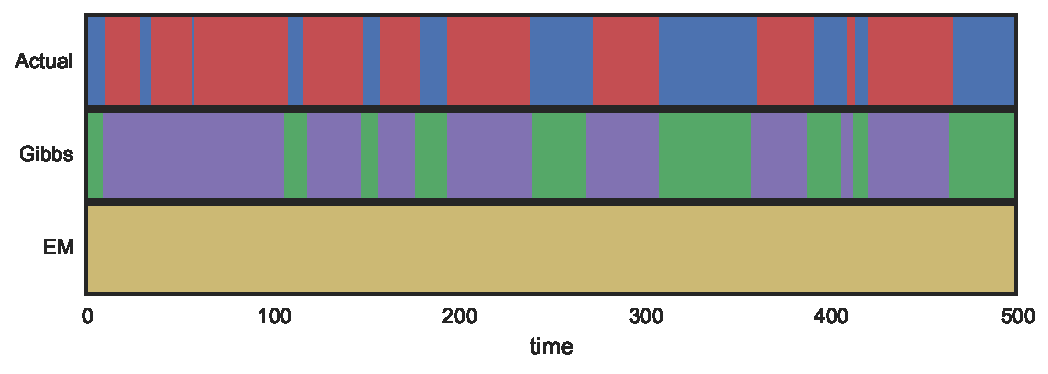
\includegraphics[width=1\textwidth]{img/trick_coin_states.pdf}
    \caption[Inferred states from trick coin example]{
        Actual state sequence and example inferred state sequences from the
        HMM fit with Gibbs sampling and EM. The HMM fit with EM
        only uses a single state to model the observed sequence.
    }
    \label{fig:trick-coin-states}
\end{figure}

For the second task 500 $(\seq{x}{1}{T}^{\text{trick}}, \seq{x}{1}{T}^\text{single})$ pairs
of sequences were generated. The ability of each model to discriminate (by comparing likelihoods)
is assessed for each pair. This same experiment was repeated 25 times using a different single
training sequence and pairs of testing sequences. Again, the \ac{HMM} fit with Gibbs sampling
significantly outperformed the \ac{HMM} fit with \ac{EM}, Figure~\ref{fig:trick-coin-disc}.

\begin{figure}[H]
    \centering
    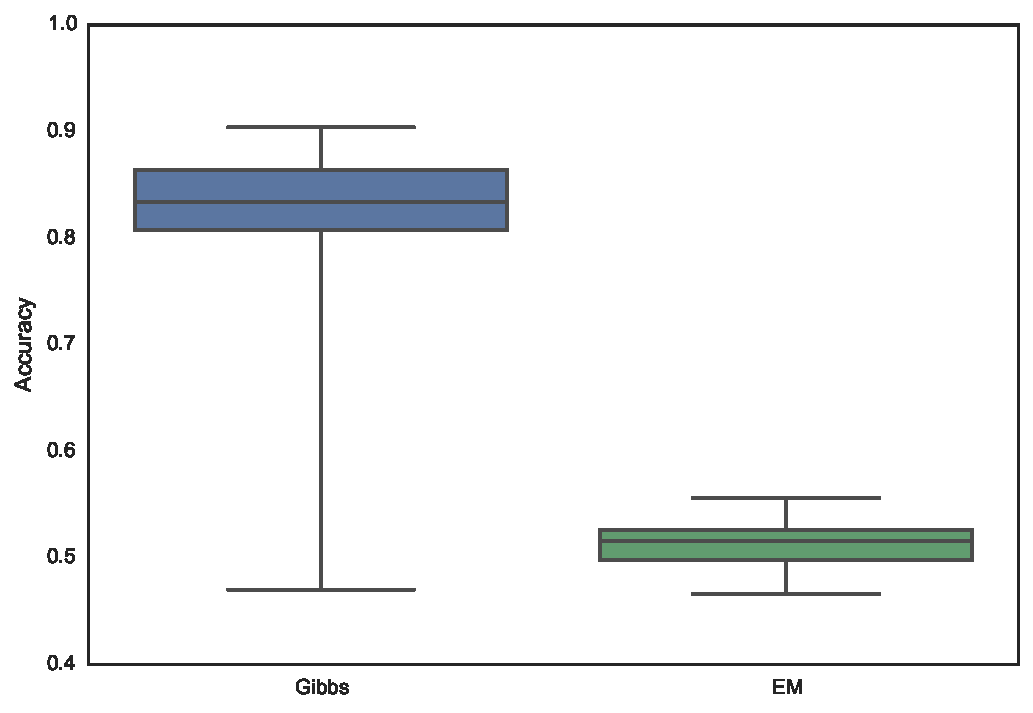
\includegraphics[width=1\textwidth]{img/trick_coin_disc_accuracy.pdf}
    \caption[Trick coin accuracy]{
        Accuracy for the trick coin discriminative task. Whiskers
        depict the maximum and minimum values.
    }
    \label{fig:trick-coin-disc}
\end{figure}

\section{Learning to Segment Repetitive Sequences}
\label{sec:Learning to Segment Repetitive Sequences}
Having demonstrated the effectiveness of the collapsed Gibbs sampling approach,
we now describe experiments which demonstrate the ability of the \ac{CHMM} to utilize its repetitive
latent structure in an artificial segmentation task. Sequences were generate by
embedding a recurrent sequence between two constant sequences and adding Gaussian random noise.
In particular an example sequence is generated from the following distribution.

\begin{align*}
    t_1 & \sim 100 \cdot \Beta(5, 5) + 10 \\
    t_2 & \sim 100 \cdot \Beta(5, 5) + 10 + t_1 \\
    t_3 & \sim 100 \cdot \Beta(5, 5) + 10 + t_2 \\
    \epsilon_t & \sim \Norm(0, 1/2),\; t = 1,\ldots,t_3 \\
    x_t &= \epsilon_t,\; t=1,\ldots,t_1 \\
    x_t &= \sin(t) + \epsilon_t,\; t=t_1+1,\ldots,t_2 \\
    x_t &= \epsilon_t,\; t=t_2 + 1,\ldots,t_3\\
\end{align*}

A model for segmenting such sequences must distinguish between the recurrent portion,
$\seq{x}{t_1+1}{t_2}$, and the constant portions, $\seq{x}{1}{t_1}$, $\seq{x}{t_2+1}{t_3}$.
More formally, each timestep $x_t$ in the sequence is annotated with a tag $a_t \in \{I, O\}$
denoting whether the sequence is \emph{in} ($I$), or \emph{out} ($O$) of the repetitive portion
of the sequence at time $t$. The annotation is similar to the BIO (begin/in/out) representation
commonly used in \ac{NLP} chunking applications~\cite{ramshaw-bio}.
\\\\
Rather than using these annotations within the learning procedure (for example, to learn a
discriminative classifier) an unsupervised approach is taken, in which only the raw sequence
is available during training. Thus the ability to discover structure in the time series rests
entirely on a priori structure built into the model itself.
\\\\
To capture this structure the prior distribution over transition matrices
(a Dirichlet distribution for each row) is split into three regime blocks.
The first and third block corresponds to a standard \ac{HMM}
in which each state may transition to every other state, the \emph{out} portions of the sequence.
The second block corresponds to the \ac{CHMM} structure in which states transition
only to themselves or their successor states, the \emph{in} portion of the sequence.
To allow movement between these blocks, transitions are added from each state in the first block
to the start state of the second block, and from the final state of the second block to each state
in the third block. Diagrammatically this results in the structure depicted below.

\begin{align*}
    \bm{\alpha} &= \left[\begin{array}{c | c | c}
        F & A_1 & \bm{0} \\\hline
        \bm{0} & S & A_2 \\\hline
        \bm{0} & \bm{0} & F
    \end{array}\right] \\
    F &= \left[\begin{array}{c c c}
        \alpha_0 & \cdots & \alpha_0 \\
        \vdots   &        & \vdots \\
        \alpha_0 & \cdots & \alpha_0
    \end{array}\right] &
    S &= \left[\begin{array}{c c c c c}
        \alpha_3 & \alpha_4 & 0        & \cdots   & 0        \\
        0        & \alpha_3 & \alpha_4 & \ddots   & \vdots   \\
        \vdots   & \ddots   & \ddots   & \ddots   & 0        \\
        0        & \cdots   & 0        & \alpha_3 & \alpha_4 \\
        \alpha_4 & 0        & \cdots   & 0        & \alpha_3
    \end{array}\right] \\
    A_1 &= \left[\begin{array}{c c c c}
        \alpha_1 & 0      & \cdots & 0 \\
        \vdots   & \vdots &        & \vdots \\
        \alpha_1 & 0      & \cdots & 0
    \end{array}\right] &
    A_2 &= \left[\begin{array}{c c c}
        0        & \cdots & 0 \\
        \vdots   &        & \vdots \\
        0        & \cdots & 0 \\
        \alpha_2 & \cdots & \alpha_2
    \end{array}\right]
\end{align*}

Here the $\alpha_i$ terms are parameters of a prior on transitions from

\begin{align*}
    \alpha_0: & \text{ an \emph{out} state to an \emph{out} state,}\\
    \alpha_1: & \text{ an \emph{out} state to an \emph{in} state,}\\
    \alpha_2: & \text{ an \emph{in} state to an \emph{out} state,}\\
    \alpha_3: & \text{ an \emph{in} state to itself,}\\
    \alpha_4: & \text{ an \emph{in} state to its successor \emph{in} state.}\\
\end{align*}

Using just 2 sample sequences and the above described prior structure with
1 \emph{out} state and 5 \emph{in} states allows the collapsed Gibbs sampler
to discover highly accurate segmentations in a completely unsupervised manner,
Figure~\ref{fig:artificial-segmentation-struct}. To demonstrate the necessity for the prior,
and rule out the possibility that the model is doing something uninteresting (such
as modeling differences in variance within the distinct regimes) the same experiment
was repeated with a standard \ac{HMM} with two states. In this case, the model is completely
unable to discover any interesting structure in the sequence,
Figure~\ref{fig:artificial-segmentation-flat}.

\begin{figure}[H]
    \centering
    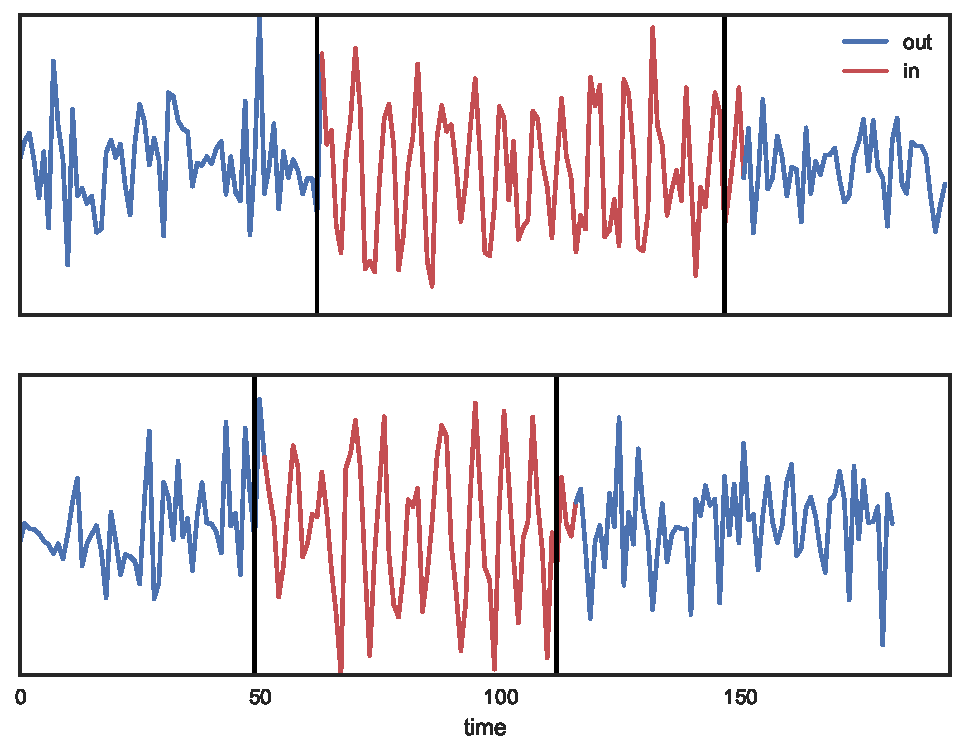
\includegraphics[width=1\textwidth]{img/artificial-segment-output-struct.pdf}
    \caption[Example segmentation of synthetic sequences with structure]{
        Unsupervised segmentation by a HMM with structured prior.
    }
    \label{fig:artificial-segmentation-struct}
\end{figure}

\begin{figure}[H]
    \centering
    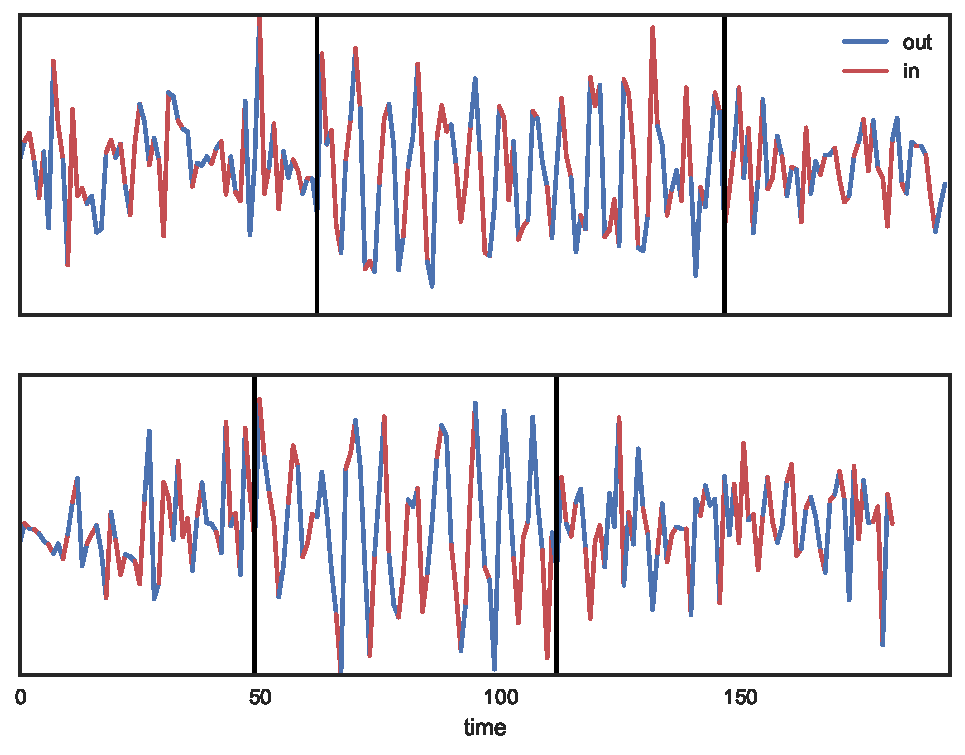
\includegraphics[width=1\textwidth]{img/artificial-segment-output-flat.pdf}
    \caption[Example segmentation of synthetic sequence without structure]{
        Unsupervised segmentation by a HMM with 2 states.
    }
    \label{fig:artificial-segmentation-flat}
\end{figure}

\section{Clustering Sequences}
\label{sec:Clustering Sequences}
The final synthetic experiment explores the Bayesian nonparametric approach outlined in
Section~\ref{sec:Mixtures of Hidden Markov Models} for the purpose of sequence clustering.
As ground truth clusters the following four recurrent functions are used.

\begin{align*}
    f_1(t) &= \sin(t) &
    f_3(t) &= \max(-2, \min(2, \tan(t/4))) \\
    f_2(t) &= \sin(t) + \sin(t/2) &
    f_4(t) &= \max(0, 2 \cos(t/ 4))
\end{align*}

An example sequence is then generated from the following process.

\begin{align*}
    t_0 & \sim \Unif({0, \ldots, 200}) \\
    t_1 & \sim \Geom(1/10) + 50 + t_0 \\
    \epsilon_t & \sim \Norm(0, 1/2) \\
    x_t &= f_k(t) + \epsilon_t,\; t=t_0,\ldots,t_1.
\end{align*}

This procedure is repeated 10 times for each $k \in \{1,2,3,4\}$ resulting in 40
total training sequences.
\\\\
Two clustering approaches are considered. The \ac{DPMoHMM} utilizes standard \acp{HMM}
as the base distribution and the \ac{DPMoCHMM} uses \acp{CHMM} as the base distribution.
The experiment is repeated 10 times and the resulting clusterings are compared using
\ac{AMI}~\cite{ami}, a version of Mutual Information corrected to adjust for chance agreements.
Figure~\ref{fig:artificial-cluster-metrics} shows that as well as increased performance,
in terms of \ac{AMI}, the \ac{DPMoCHMM} finds the correct number of clusters in 80\% of experiments.
This is in contrast to the \ac{DPMoHMM}, which is unable to find the actual number of clusters in any
of the experiments.

\begin{figure}[H]
    \centering
    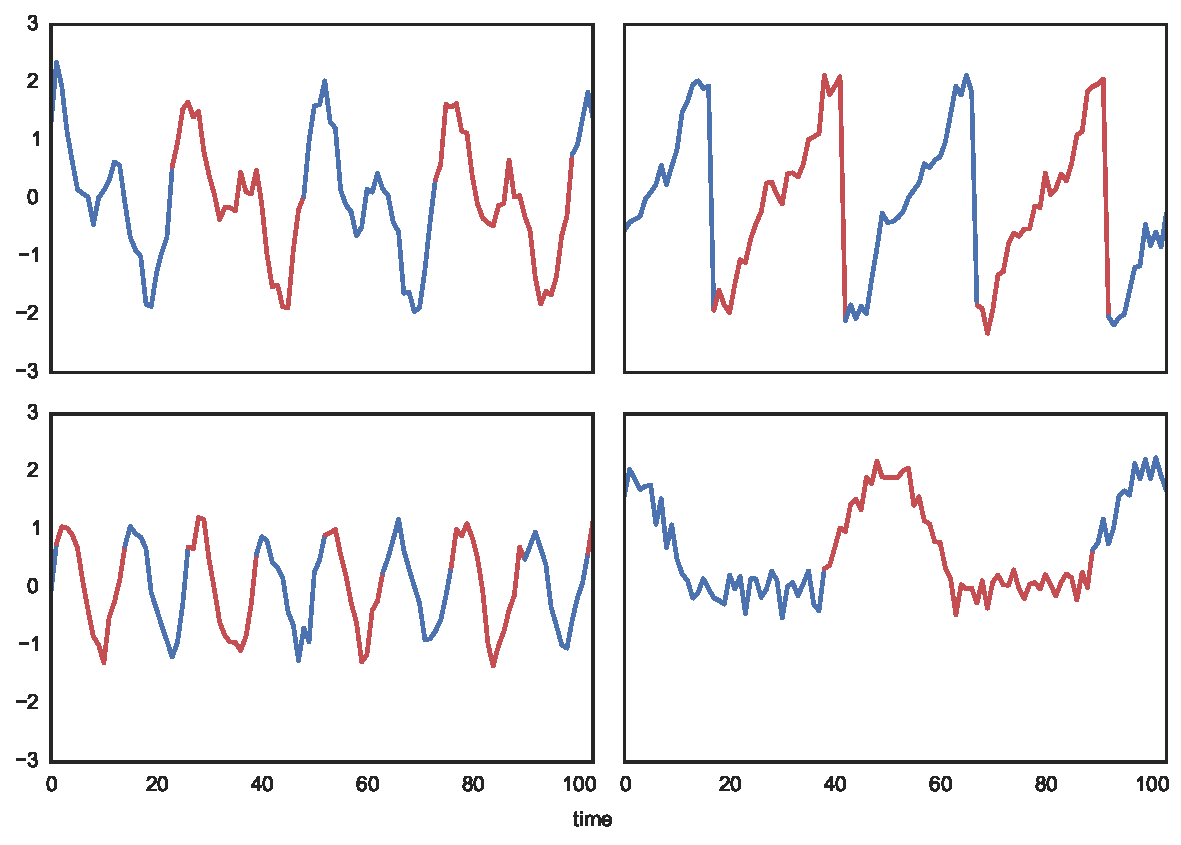
\includegraphics[width=0.8\textwidth]{./img/artificial-clusters.pdf}
    \caption[Visualization of synthetic sequence clusters]{
        Example from each cluster and recurrent structure
        discovered by the \ac{DPMoCHMM}.
    }
    \label{fig:artificial-clusters}
\end{figure}

\begin{figure}[H]
    \centering
    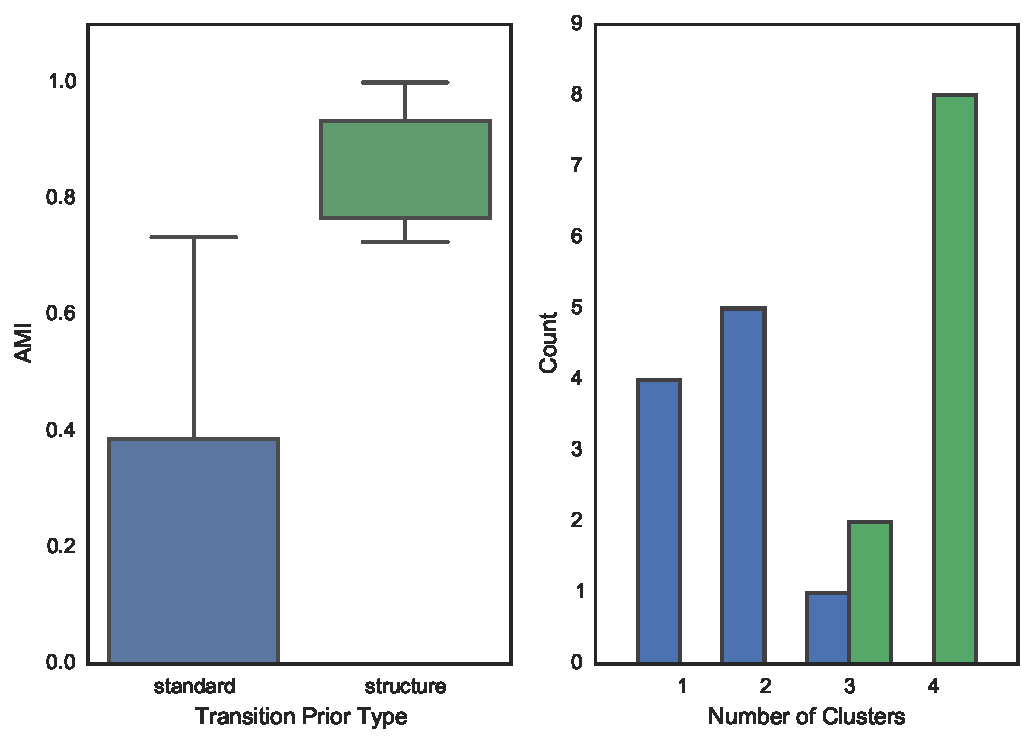
\includegraphics[width=\textwidth]{./img/artificial-cluster-results.pdf}
    \caption[Synthetic sequence clustering results]{
        Results from clustering artificial sequences.
        Comparison of Adjusted mutual information and number of discovered
        clusters with (green) and without (blue) structured transition prior.
    }
    \label{fig:artificial-cluster-metrics}
\end{figure}


\chapter{Segmented Exercise Classification}
\label{chap:Segmented Exercise Classification}
An obvious precursor to classifying each timestep of an entire routine is to classify the hand segmented
exercises into 1 of $K$ mutually exclusive exercise classes. This task is significantly easier than
than the full routine classification task since several simplifying assumptions can be made. First,
we can assume each sequence belongs to a single class. Second, we can assume each class is approximately
equally likely a priori and avoid dealing with the class imbalance problem that arises when working with
full routines, which are overwhelmingly dominated by \emph{rest}.

\section{Setup}
For training and evaluation purposes we used a random train/test split of the
available data (approximately 70\% of the data was used for training and the remaining
30\% was used for testing), randomized over users. Keeping the set of users in these sets
disjoint is particularly important as it mimics the situation one would actually encounter
if deploying such a system. Classifier hyperparameters were set using grid search performed on an
analogous split of the training data. Table~\ref{table:segment-dataset} summarizes the splits.

\begin{table}[ht]
    \centering
    \begin{tabular}{l r r}\hline
    & \textbf{Train} &\textbf{Test} \\\hline
    Users & 85 & 37\\
    Classes & 50 & 50\\
    Activities & 3364 & 1382\\
    Repetitions & 28476 & 12396\\
    Minutes of Data & 1247 & 557\\
    \end{tabular}
    \caption[Summary of segment classification dataset]{
        Summary of segment classification dataset.
    }
    \label{table:segment-dataset}
\end{table}

\section{Models}
The proposed \ac{CHMM} was compared to a Structured Perceptron~\cite{perceptron-collins}
and a strong performing system heavily influenced from the activity recognition literature~\cite{ms-activity}.
As only sequences with a single label are considered in this experiment, a voting procedure is used
to aggregate predictions for individual time steps to produce the final classification for both
the Random Forest and Structured Perceptron. Note that this gives an unfair advantage to these
models. In a real world activity classification setting one would not a priori have knowledge of
the bounds (segmentation) over which to aggregate votes.

\subsection{Baseline from Literature}
A classifier inspired by~\cite{ms-activity} (discussed in Section~\ref{sec:HAR Related Work})
was developed to provide a strong performing baseline. Significantly better results were
obtained on the data considered here using a Random Forest rather than a \ac{SVM},
and only the performance of the former is reported.
This discrepancy is likely due to \cite{ms-activity} utilizing a number of heuristic feature
partitioning schemes which were not able to be replicated in this work.
\\\\
The following features were computed over 4 second windows (60 timesteps)
for each of the 3 accelerometer and 3 gyroscope axis:
\begin{itemize}[nosep]
    \item The number of peaks in the autocorrelation function.
    \item The height of the first peak of the autocorrelation function after crossing zero.
    \item The maximum value of the autocorrelation function.
    \item The mean of the signal.
    \item The standard deviation of the signal.
    \item The norm of the signal.
    \item The magnitude of the power spectrum summed across 10 linearly spaced bands.
\end{itemize}
The free software scikit-learn \cite{scikit-learn} was used
to estimate parameters of the Random Forest. Grid search was performed
over the following hyper-parameters:\footnote{
Best performing settings on the validation set are noted in bold.
}
\begin{itemize}[nosep]
    \item The number of trees in the forest: $(25, 50, \mathbf{100})$.
    \item The minimum number of samples in each leaf node: $(2, \mathbf{5}, 10)$.
    \item The maximum depth of each tree: $(10, 20, \mathbf{none})$.
    \item The maximum number of features considered for each split: $(\mathbf{\sqrt{d}}, all)$.
    \item The spit evaluation function: \textbf{Gini impurity} or information gain.
\end{itemize}

\subsection{Structured Perceptron}
The Structured Perceptron is a discriminative analog of a \ac{HMM}.
It is worth noting this claim is somewhat tenuous, and it might
be considered more appropriate to say this is only true of the closely
related \ac{CRF}, which models $P(Y|X)$ as opposed to a \ac{HMM}
which models $P(Y,X)$. Regardless, both are chain structured discriminative
models which avoid the local normalization problems, \emph{label bias}, associated
with \acp{HMM} and \acp{MEMM} \cite{lafferty-crf}.
\\\\
Despite avoiding the label bias problem, the gradient based algorithms frequently
used for training such models do not easily extend to models with latent variables.
As latent variables offer a significant amount of flexibility this is a potential
drawback for such models.
\\\\
CRFSuite \cite{CRFsuite}, a free structured linear model implementation, was used
for training the Structured Perceptron. \acp{CRF} and Structured Perceptrons
with Passive Aggressive weight updates were also evaluated for several settings of
hyper-parameters. The Averaged Structured Perceptron obtained lower overall
error on the data considered here. The Averaged Structured Perceptron has no hyperparameters.

\subsection{Mixtures of Cyclic Hidden Markov Models}
The conditional probability of a sequence belonging to one of the
$K$ exercise classes can be modeled by forming a mixture of \acp{CHMM}
and calculating the predictive distribution as
\[
    P(k \mid \seq{x}{1}{T}, \seq{y}{1}{T}) \propto P(k)P(\seq{x}{1}{T}, \mid k)
\]
where $P(k)$ is prior probability of exercises $k$.
In these experiments, $P(k) = 1 / K$ is fixed. Given labeled segments,
parameter estimation of the component \acp{CHMM} can be carried
out independently. Two methods of parameter estimation are considered.
\\\\
The first method searches for \ac{MAP} parameters using Viterbi Training
\cite{segmental-kmeans}. Viterbi Training seeks model parameters which maximize
the probabilities of the most likely latent sequences given the observed sequences,
rather than parameters that maximize the probability of the observed sequences as is done
in classical \ac{EM}. This criteria was found to perform slightly better than the typical
\ac{EM} approach for estimating \ac{HMM} parameters. Recent work provides both empirical
and theoretical support for this observation, especially when fitting highly misspecified models,
and/or in cases in which the final performance will be measured using
the MAP state sequence. For further discussion on this subject we defer the interested reader
to Sections 7 and 8 of \cite{viterbi-em} as well as \cite{estimate-wrong}.
\\\\
The second method is based on the collapsed block Gibbs sampling approach outlined in
Section~\ref{sec:A Block Collapsed Gibbs Sampler for Hidden Markov Models}.
The MAP sampled assignment is used to produce a point estimate of the parameters.

\section{Results}
Table~\ref{table:segment-results} gives train and test set accuracy numbers for the
considered classification methods. In general the Random Forest outperforms the other
models in terms of raw accuracy, although the \ac{MoCHMM} is quite competitive.
The Structured Perceptron significantly under performs the other models,
likely due to being restricted to linear decision boundaries as noted above.
\\\\
The same experiments as above were repeated for the Random Forest and \ac{MoCHMM} fit with
the collapsed Gibbs sampler, but this time including a number of \emph{rest} sequences
equal the most frequent activity. While the accuracy of the Random Forest degrades in this regime,
surprisingly the accuracy of the \ac{MoCHMM} increases. Inspecting performance for just the \emph{rest} class
reveals this is at least in some part due to the \ac{MoCHMM} doing a better job of modeling
the \emph{rest} class, the last two columns of Table~\ref{table:segment-results-rest}.
The lower recall number for the Random Forest imply that approximately 25\% of the \emph{rest}
sequences are misclassified as an activity.
\begin{table}[ht]
    \centering
    \begin{tabular}{l r r}\hline
    \textbf{Classifier} & \textbf{Train Accuracy} &\textbf{Test Accuracy} \\\hline
    MAP Baseline & 0.043 & 0.037 \\
    Structured Perceptron & 0.681 & 0.598 \\
    Random Forest & 0.997 & \textbf{0.827} \\
    MoCHMM (Gibbs) & 0.848 & 0.775 \\
    MoCHMM (Viterbi) & 0.837 & 0.762 \\
    \end{tabular}
    \caption[Performance on the segmented exercise task]{
        Segment classification performance of different classifiers.
    }
    \label{table:segment-results}
\end{table}
\begin{table}[ht]
    \centering
    \begin{tabular}{l r r r r r}\hline
    \textbf{Classifier} & \textbf{Train Acc.} & \textbf{Test Acc.} & \textbf{F1}    & \textbf{Precision} & \textbf{Recall} \\\hline
    Random Forest       & 0.995               & \textbf{0.81}      & 0.789          & \textbf{0.925}     & 0.755 \\
    MoCHMM (Gibbs)       & 0.829               & 0.799              & 0.790          & 0.81               & \textbf{0.829} \\
    \end{tabular}
    \caption[Performance on the segmented exercise task with \emph{rest}]{
        Segment classification performance including the \emph{rest} class.
        The F1-score is reported as a macro (unweighted) average of the individual classes.
        Precision and recall are for \emph{rest} only.
    }
    \label{table:segment-results-rest}
\end{table}

Another important observation is the significant performance degradation of the Random Forest
on unseen data. Performance of the Random Forest decreases by 17\% and 18.5\% on unseen data
for the two experiments described here, a significant amount compared to the more mild 8\% and 4\%
percent decreases obtained by the \ac{MoHMM}. Several attempts were made to combat overfitting in
the Random Forest, largely by reducing the complexity of the individual ensemble members, however
in all cases this resulted in decreased test performance.


\chapter{Segmenting Exercises}
\label{chap:Segmenting Exercises}
The strong performing baseline classifier from Chapter~\ref{chap:Segmenting Exercises} has the disadvantage
that it requires relatively tight ground truth segmentations. Significant performance degradation
was observed when many examples had large portions of \emph{rest} leading and/or trailing the activity.
Given the inherent non-sequential treatment of the input, this observation should not be surprising.
Analogous behavior would be observed in a \ac{iid} classification setting if many
negative samples (\emph{rest}) were incorrectly labeled positively (\emph{exercise}).
In contrast the \ac{CHMM} can perform this segmentation in an unsupervised manner simply by inspecting the
inferred latent states.

\section{Unsupervised Segmentation}
\label{sec:Unsupervised Segmentation}
The system described in Section~\ref{sec:Learning to Segment Repetitive Sequences} was applied unmodified
to the task of segmenting exercise boundaries. For each class, the parameters of a single \ac{CHMM}
were estimated using all available data for that class. The resulting parameters were then
used to infer the \ac{MAP} latent state sequences $\seq{y}{1}{T}$ for each sequence.
\\\\
Using the terminology introduced previously, let $\mathcal{O},\; \mathcal{I} \subseteq Y$
denote the set of \emph{out} states and \emph{in} states respectively.
Then the inferred start and stop times of the activity are given by

\begin{align*}
    t_\text{start} &= \min_t\{ y_t \in \mathcal{I}\} \\
    t_\text{stop} &= \min_t\{y_{t-1} \in \mathcal{I} \land y_t \in \mathcal{O}\}.
\end{align*}

Unfortunately, as the only annotations available are the ones which are to be corrected,
it is difficult to define a performance metric to quantitatively evaluate the resulting segmentations.
Instead, visual inspection of a random subset of exercises was used to qualitatively assess model performance.

\begin{figure}[H]
    \centering
    \begin{subfigure}{0.82\textwidth}
        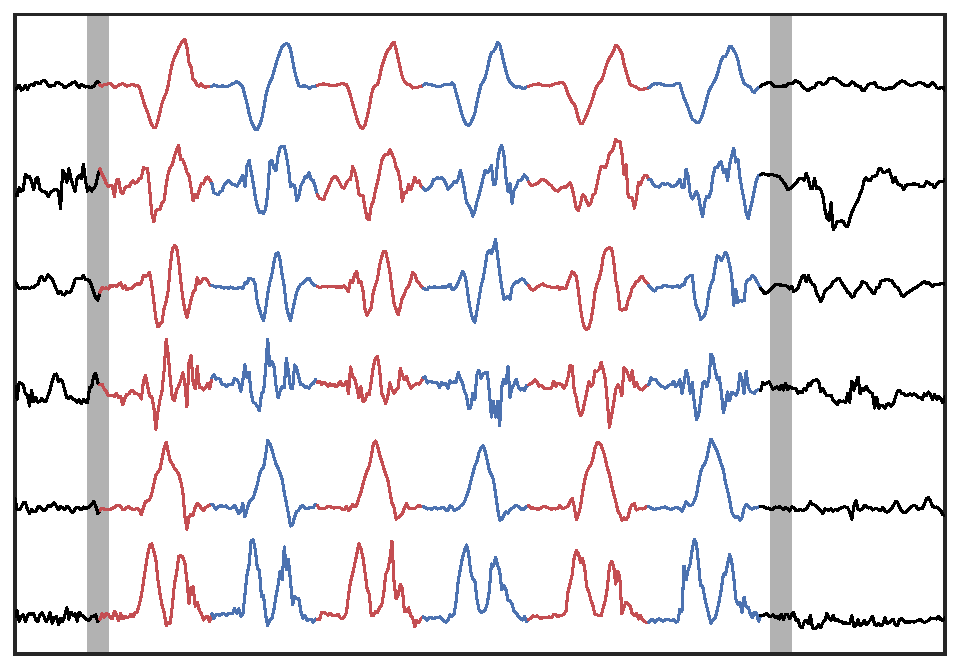
\includegraphics[width=\textwidth]{img/segmentation/alt_db_bicep_curl.pdf}
        \caption{Alternating Dumbbell Bicep Curls.}
        \label{fig:actseg:alt-db-curl}
    \end{subfigure}
\end{figure}

\begin{figure}[H]
    \centering
    \ContinuedFloat
    \begin{subfigure}{0.82\textwidth}
        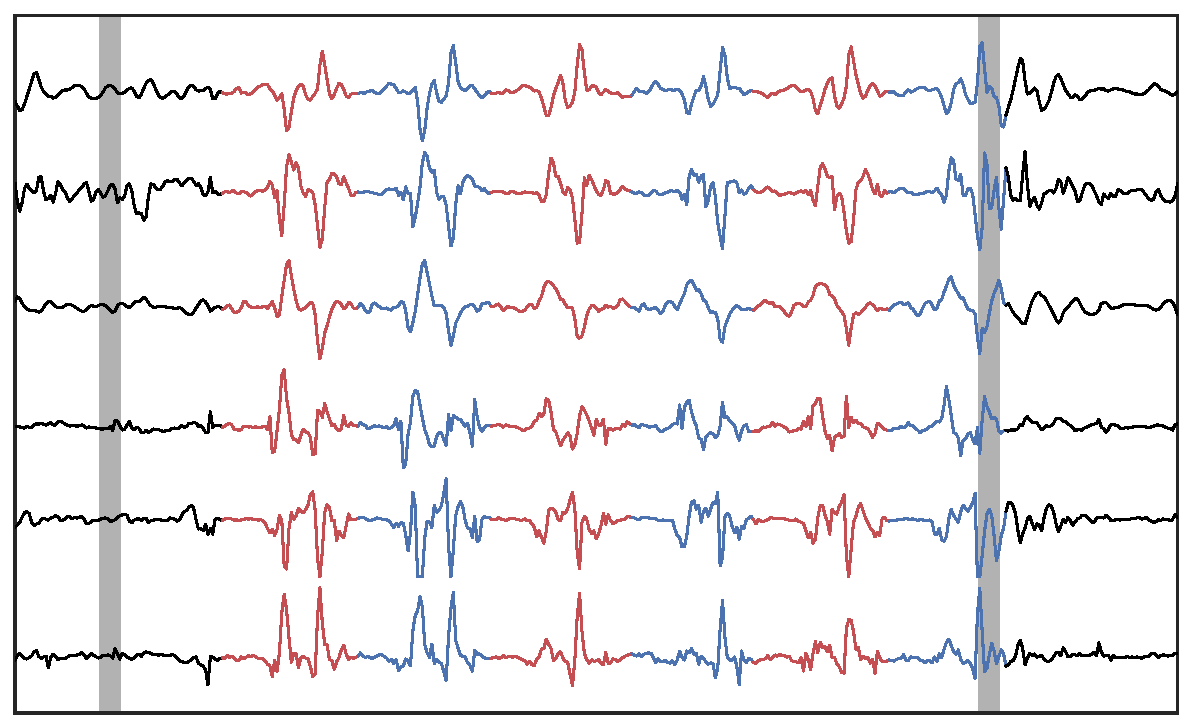
\includegraphics[width=\textwidth]{img/segmentation/burpee.pdf}
        \caption{Burpees.}
        \label{fig:actseg:burpee}
    \end{subfigure}
\end{figure}

\begin{figure}[H]
    \centering
    \ContinuedFloat
    \begin{subfigure}{0.82\textwidth}
        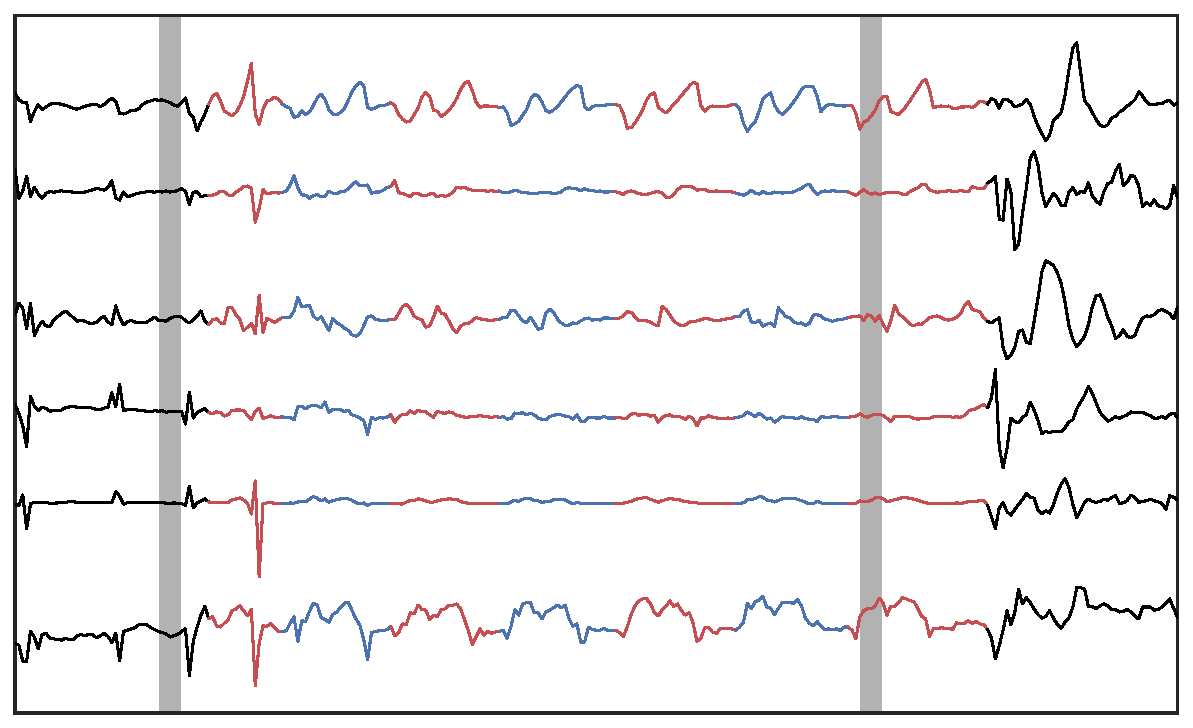
\includegraphics[width=\textwidth]{img/segmentation/push_up.pdf}
        \caption{Push-Ups.}
        \label{fig:actseg:push-up}
    \end{subfigure}
    \caption[Unsupervised exercise segmentation]{
        Visualization of segmentations produced by the CHMM.
        Large grey bars denote observer annotations. Parts of the sequence drawn
        in black correspond to \emph{out} predictions, and parts drawn in color
        correspond to \emph{in} predictions. Red and blue highlight the repetitive structure
        discovered by the algorithm. The ability of the CHMM to correct erroneous
        annotations is clearly visible in (\subref{fig:actseg:burpee}) and (\subref{fig:actseg:push-up}).
    }
    \label{fig:actseg}
\end{figure}

\section{Results}
For a majority of inspected sequences the algorithm was able to produce nearly
equivalent or superior segmentations when compared to those produced by the observer.
Figure~\ref{fig:actseg} visually contrasts the segmentations produced by the \ac{CHMM}
and those produced by the exercise observer. the ability of the \ac{CHMM} to produce
superior annotations is particularly prevelant in Figures~\ref{fig:actseg:burpee}
and~\ref{fig:actseg:push-up}.
\\\\
The ability to ``clean up'' erroneous or noisy segmentations puts the \ac{CHMM}
in a unique position. As well as being able to form the basis of a competitive classifier,
it can also serve as a valuable preprocessing tool to produce more accurate examples in
classification settings where discriminative models ultimately prevail.

\chapter{Clustering Exercise Types}
\label{chap:Clustering Exercise Types}
The experiments presented in Chapter~\ref{chap:Segmented Exercise Classification}
and Chapter~\ref{chap:Segmenting Exercises} assume labels for the type of exercises
being performed are given during the parameter estimation phase. This Chapter explores
the scenario when the type of exercise being performed, and number of unique types is unknown.
\\\\
Given these assumptions, a natural task is to attempt to partition the
set of individual sequences into clusters. Ideally these clusters would
correspond to the types of exercise being performed. Since the number of
unique types is also unknown the Bayesian nonparametric approach described in
Section~\ref{sec:Mixtures of Hidden Markov Models}, and utilized to cluster
artificial data in Section~\ref{sec:Clustering Sequences}, is used. To assess the
value of the \ac{CHMM} structure experiments are carried out using either a \ac{CHMM}
or \ac{HMM} base distribution.

\section{Experiment Setup}
The ability of the \ac{DPMoCHMM} and \ac{DPMoHMM} to cluster exercises is assessed
using three and nine exercises classes. To measure the effect of dataset size the number of
exercise sequences used to estimate model parameters is varied as well. For the experiments
carried out with 3 classes 10, 20, 40, 60, and 100 example sequences from each class are used,
resulting in 30, 60, 120, 180, and 262 total samples\footnote{For some exercise we did not
have 100 samples, resulting in 262 samples rather than 300}. For the experiments carried out with
9 classes 10 and 90 example sequences from each class are used, resulting in 90 and 360 total samples.
\\\\
For each experimental setup (number of classes and number of sample sequences)
15 models of each type were fit to allow averaging performance metrics and assess model stability.
The parameters of each model are fit using a different randomly selected subset of the available data,
although the same random subsets are used for both the \ac{DPMoHMM} and \ac{DPMoCHMM} to enable
staightforward comparison. Table~\ref{table:cluster-experiment} lists the exercises used.

\begin{table}[H]
    \centering
    \begin{tabular}{r | p{8cm}}\hline
    \textbf{Classes} & \textbf{Exercises} \\\hline
    3 &  burpees, sit-ups, dumbbell lateral raises\\\hline
    9 & dumbbell tricep extension, jumping jacks, burpees, sit-ups, dumbbell lateral raises, box jumps, alternating dumbbell bicep curls, push-ups, pull-ups\\
    \end{tabular}
    \caption[Exercises used in clustering experiments]{
        Exercises used in clustering experiments.
    }
    \label{table:cluster-experiment}
\end{table}

\section{Results}
In both the three and nine class experiments the \ac{DPMoCHMM}
is able to produce fairly accurate clusterings as measured by
\ac{AMI}, and in all cases outperforms the \ac{DPMoHMM}, Table~\ref{table:cluster-types-ami}.
This provides further support for the benefit of incorporating prior
structure into the model. There also appears to be a much stronger
relationship between \ac{AMI} and the complete data log likelihood for the
\ac{DPMoCHMM} than the \ac{DPMoHMM}, Figure~\ref{fig:cluster-type-correlation}.
This is especially important since one would not have access to the label required
to compute \ac{AMI} in a real world clustering scenario, and alternate measures of performance,
such as likelihood, would need to be used to evaluate model performance.

\begin{table}[H]
    \centering
    \begin{tabular}{r | r | c r r | c r r}\hline
    \multirow{2}{*}{\textbf{Classes}} & \multirow{2}{*}{\textbf{Size}} & \multicolumn{3}{c |}{\textbf{Flat}} & \multicolumn{3}{c}{\textbf{Cycle}} \\\cline{3-8}
    & & AMI & Fail & Success & AMI & Fail & Success \\\hline
    $3$ & $30$ & $0.30 \pm 0.27$ & $6$ & $2$ & $0.56 \pm 0.28$ & $2$ & $7$\\
    $3$ & $60$ & $0.38 \pm 0.21$ & $3$ & $0$ & $0.65 \pm 0.13$ & $0$ & $11$\\
    $3$ & $120$ & $0.23 \pm 0.25$ & $8$ & $0$ & $0.59 \pm 0.25$ & $1$ & $8$\\
    $3$ & $180$ & $0.30 \pm 0.25$ & $6$ & $1$ & $0.69 \pm 0.24$ & $1$ & $11$\\
    $3$ & $262$ & $0.41 \pm 0.31$ & $5$ & $4$ & $0.65 \pm 0.14$ & $0$ & $8$\\\hline
    $9$ & $90$ & $0.30 \pm 0.11$ & $0$ & $0$ & $0.49 \pm 0.07$ & $0$ & $1$\\
    $9$ & $360$ & $0.34 \pm 0.13$ & $0$ & $0$ & $0.62 \pm 0.07$ & $0$ & $10$\\
    \end{tabular}
    \caption[Unsupervised clustering performance]{
        Comparison of unsupervised clustering with \ac{HMM} and \ac{CHMM} base distributions.
        Reported AMI is the mean $\pm$ 1 standard deviation. The fail and success columns count
        the number of runs (of 15) resulting in an AMI less than $0.1$ and greater than $0.6$ respectively.
        The model using \ac{CHMM} base distributions consistently has higher performance overall,
        more successful runs, and is less prone to failure in the 3 class case.
    }
    \label{table:cluster-types-ami}
\end{table}

As well as \ac{AMI} the resulting clusters were also assessed in terms of
supervised accuracy. To do so each cluster was assigned the label of the most
frequently appearing exercise class within that cluster. The resulting confusion
matrices and raw accuracies are given in Figure~\ref{fig:cluster-type-confusion}.
Although such numbers are not meaningful on their own, putting every sample in its
own cluster would result in 100\% accuracy, Figure~\ref{fig:cluster-type-counts} shows that
this is not the case in the experiments presented here.
\\\\
Although the results presented here are quite positive, there are several ways in
which the \ac{DPMoCHMM} does not perform adequately. The first, and most disheartening,
is largely a failure of the sampler. Occasionally the sampler would get stuck in poor
initial clusterings from which it was unable to escape. Typically this resulted in all
sequences being assigned a single cluster. This is not entirely surprising, considering that
the sampler is unable to move multiple sequences in a single step. An attempt to approximately
count the number of such failures are given in the \emph{Fail} column in Table~\ref{table:cluster-types-ami}.
\\\\
The second noteable point of failure is the inability of the sampler to discover the correct
number of true exercises, especially in the nine class case, Figure~\ref{fig:cluster-type-counts}.
This is likely due to the mismatch between the actual distribution of clusters and the
Dirichlet process. Replacing the Dirichlet process with other stochastic pocesses which
allow more control over tail behavior, such as the Pitman-Yor process \cite{pitman-yor-teh},
is a promising direction for future research.

\begin{figure}[H]
    \centering
    \begin{subfigure}{\textwidth}
        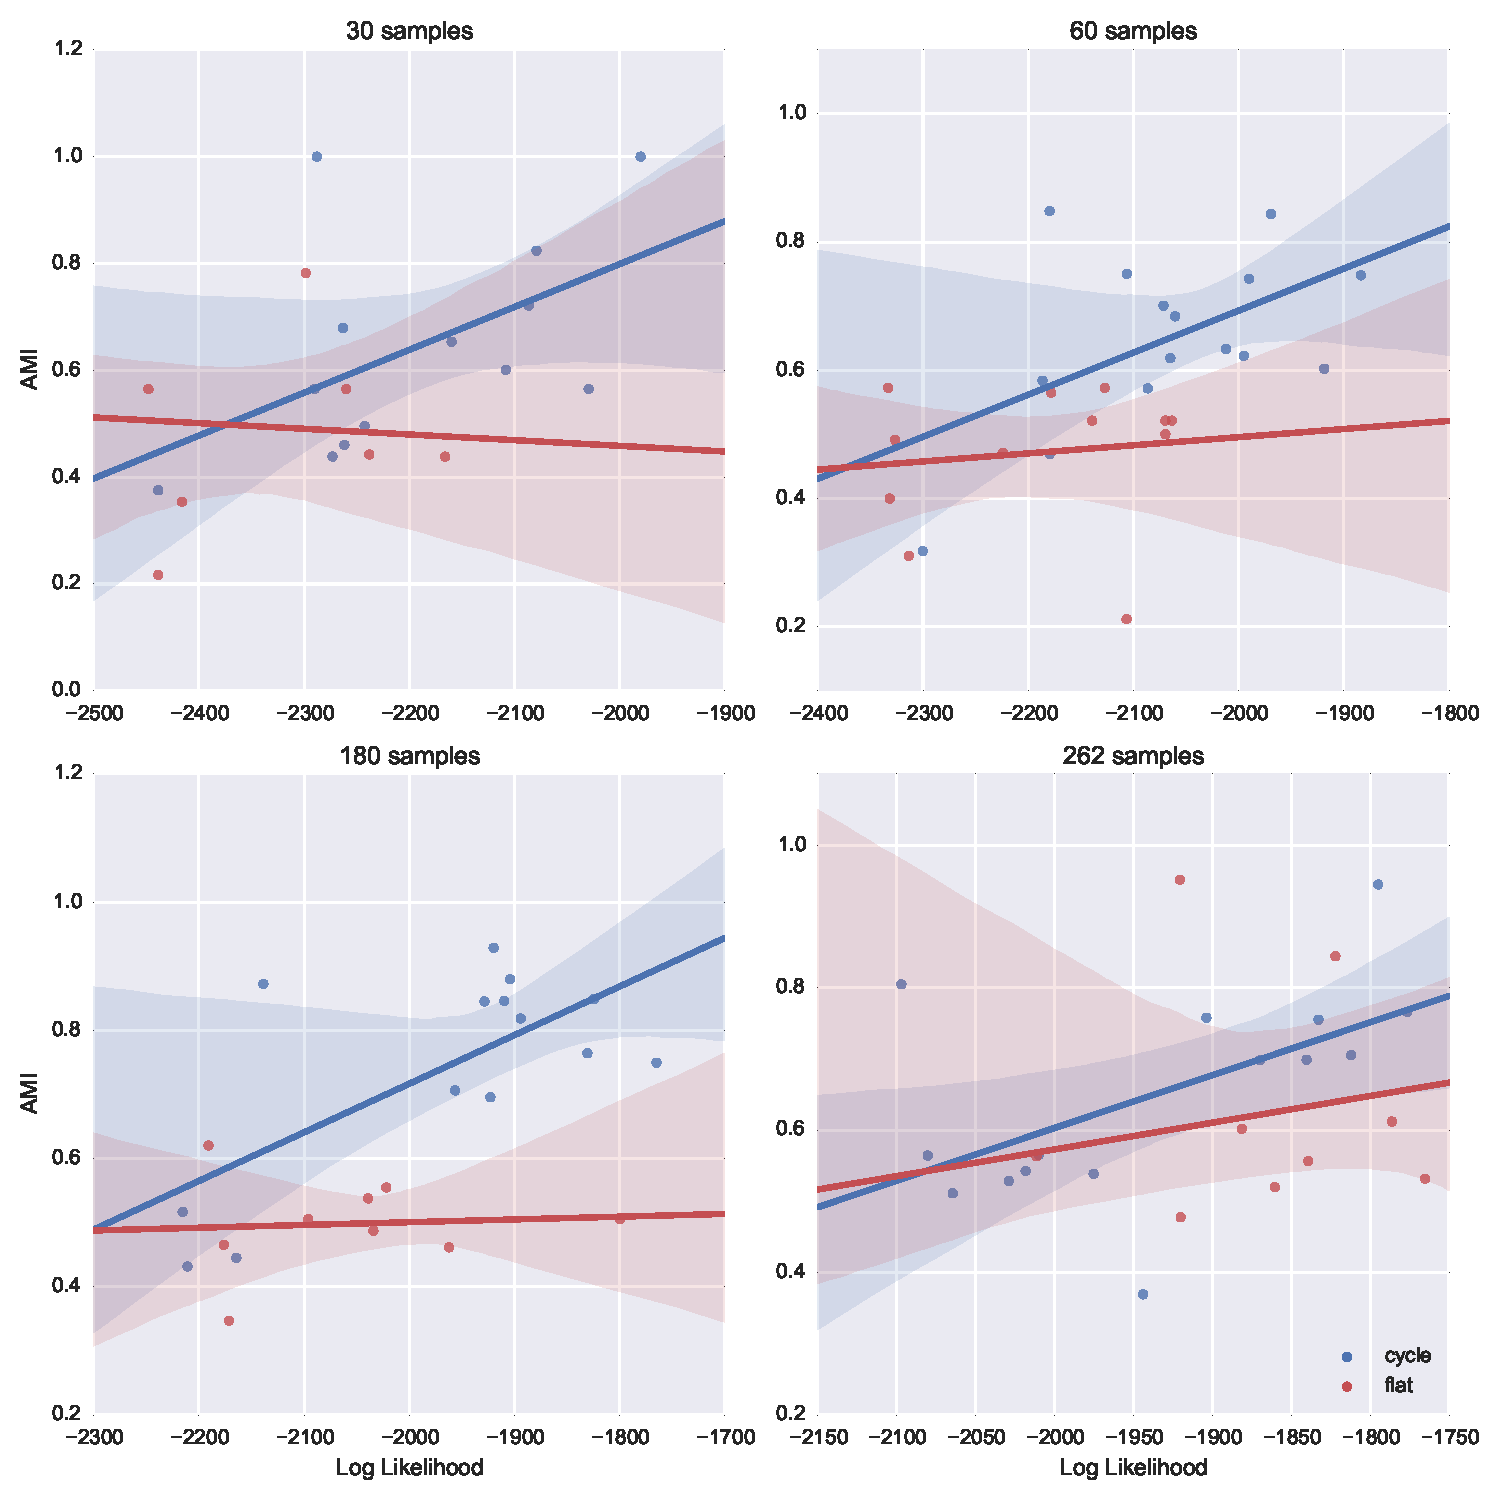
\includegraphics[width=\textwidth]{img/clustering.types/cluster-correlation.pdf}
        \caption{Three Exercises}
        \label{fig:cluster-type-confusion-3}
    \end{subfigure}
\end{figure}

\begin{figure}[H]
    \centering
    \begin{subfigure}{\textwidth}
        \includegraphics[width=\textwidth]{img/clustering.types/large-cluster-correlation.pdf}
        \caption{Nine Exercises}
        \label{fig:cluster-type-confusion-9}
    \end{subfigure}
    \caption[Relationship between log likelihood and AMI]{
        Relationship between joint log likelihood and clustering performance as measured
        by AMI for various number of sample seqeunces. Solid lines give best linear fit
        to the observed data. Shaded regions depict 95\% confidence intervals computed using
        5,000 bootstrap resamples. As can be seen, there is a much stronger trend for higher
        log likelihood to result in increased performance as measured by AMI when using a
        \ac{CHMM} (blue) base distribution than when using a standard \ac{HMM} (red).
    }
    \label{fig:cluster-type-correlation}
\end{figure}

\begin{figure}[H]
    \centering
    \begin{subfigure}{\textwidth}
        \includegraphics[width=\textwidth]{img/clustering.types/cluster-counts.pdf}
        \caption{Three Exercises.}
        \label{fig:cluster-type-counts-3}
    \end{subfigure}
    \begin{subfigure}{\textwidth}
        \includegraphics[width=\textwidth]{img/clustering.types/large-cluster-counts.pdf}
        \caption{Nine Exercises.}
        \label{fig:cluster-type-counts-9}
    \end{subfigure}
    \caption[Number of discovered clusters]{
        Histogram of the number of clusters discovered by the DPMoHMM (red) and DPMoCHMM (blue)
        when using 3 (\subref{fig:cluster-type-counts-3}) and 9 (\subref{fig:cluster-type-counts-9})
        different exercises.
    }
    \label{fig:cluster-type-counts}
\end{figure}

\begin{figure}[H]
    \centering
    \begin{subfigure}{0.5\textwidth}
        \includegraphics[width=\textwidth]{img/clustering.types/cluster-confusion-3.pdf}
        \caption{Three Exercises.}
        \label{fig:cluster-type-confusion-3}
    \end{subfigure}
    \begin{subfigure}{\textwidth}
        \includegraphics[width=\textwidth]{img/clustering.types/cluster-confusion-9.pdf}
        \caption{Nine Exercises.}
        \label{fig:cluster-type-confusion-9}
    \end{subfigure}
    \caption[Clustering confusion matrices]{
        Confusion matrices for the DPMoCHMM using 3 and 9 exercises classes.
        Each cluster is assigned the label of the most frequently appearing class.
        The resulting accuracies from upper left to lower right in
        (\subref{fig:cluster-type-confusion-3}) are 76\%, 89\%, 87\%, and 87\%,
        and from left to right in (\subref{fig:cluster-type-confusion-9}) are
        61\% and 69\%.
    }
    \label{fig:cluster-type-confusion}
\end{figure}


\chapter{Conclusions and Future Directions}
\label{chap:Conclusion}
This thesis introduced the \ac{CHMM}, a generative model specifically designed to
capture repetitive structure in time series. In contrast to much work, the \ac{CHMM}
is a restriction, rather than an elaboration, of a popular and well known Machine Learning
technique, the \ac{HMM}. Restricting capacity in such a way that a model is encouraged to use
its remaining capacity to discover structure was empirically shown to be a powerful technique
through classification, segmentation, and clustering experiments with real world time series data.
In Chapter~\ref{chap: A Generative Model for Repetitive Sequences} the \ac{CHMM} is motivated
by an automata theoretical analogy. The use of similar techniques to capture other types of
structure and in other \acp{PGM} is an interesting direction for future research.
\\\\
To cluster time series with an unknown number of types, Dirichlet process mixtures of \acp{HMM}
were also introduced. A novel collapsed block Gibbs sampler was derived to support inference in this model.
Due to working exclusively in the collapsed space, this sampler is able to simultaneously update the
cluster assignment and descendent latent states associated with a particular example. This technique is likely to be
useful in other mixture type models which feature a strong coupling between the mixture assignment
and latent variables of the base distribution.
\\\\
Despite performing well in the task considered here, the proposed sampler occasionally becomes stuck
in poor modes when applied to Dirichlet process mixture models. The analysis carried out in
Chapter~\ref{chap:Clustering Exercise Types} suggest several ways to overcome this limitation.
Due the the success of most runs, methods featuring multiple independent chains starting from
different random initializations are especially promising. This includes techniques such
as parallel tempering~\cite{learn-neighbor-mcmc} and tempered transitions~\cite{neal-tempered},
which are well suited to dealing with poor mixing in multi-modal settings.

\bibliographystyle{plain}
\bibliography{tllake.thesis}

\end{document}
